\documentclass[12pt]{report}

\usepackage{listings}
\usepackage{float}
\usepackage{booktabs}
\usepackage{amssymb}
\usepackage{subcaption}
\usepackage{graphicx}
\graphicspath{{images/}}

\input{../stile_appunti.sty}
\lstset{style=stile-listings}

\begin{document}
	
	\generaFrontespizio{Algoritmi 2}{2026}{Paul Joseph Wollan}{m}

	\chapter{Teoria dei Grafi}
	
	\begin{definizione}{Grafo}{}
		Un \textbf{grafo} è una coppia $G = (V, E)$, dove:
		\begin{itemize}
			\item $V$ rappresenta l'insieme dei \textbf{vertici} (o nodi).
			\item $E$ rappresenta l'insieme degli \textbf{archi} (o lati). Matematicamente parlando, un arco è a sua volta una coppia di valori $(v_1, v_2)$, dove $v_1, v_2$ sono de vertici del grafo.
		\end{itemize}
		Per comodità di notazione, nel corso del manuale denoteremo con $n = |V|$ il numero dei vertici e con $m = |E|$ il numero degli archi.
	\end{definizione}
	
	A titolo esemplificativo, consideriamo la seguente rappresentazione grafica di un grafo:
	
	\begin{center}
		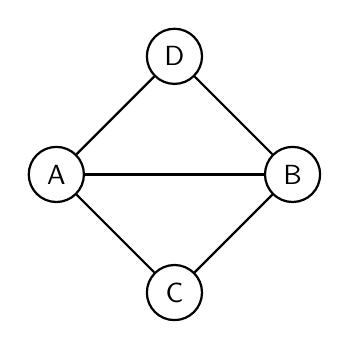
\begin{tikzpicture}[thick]
			% Definizione dello stile per tutti i nodi di questo grafo
			\tikzset{nodo/.style={circle, draw, minimum size=0.7cm, inner sep=0pt, font=\sffamily}}
			
			% Nodi posizionati in modo più ampio e simmetrico
			\node[nodo] (A) at (0, 1.5) {A};
			\node[nodo] (B) at (3, 1.5) {B};
			\node[nodo] (C) at (1.5, 0) {C};
			\node[nodo] (D) at (1.5, 3) {D};
			
			\draw (A) -- (B);
			\draw (A) -- (C);
			\draw (B) -- (C);
			\draw (A) -- (D);
			\draw (B) -- (D);
		\end{tikzpicture}
	\end{center}
	
	Riguardo agli archi, potremmo avere anche un orientamento.
	\begin{definizione}{Grafo diretto (o orientato)}{}
		Un grafo si dice \textbf{diretto} o \textbf{orientato} se ciascuno dei suoi archi ha un orientamento, cioè punta specificatamente verso un dato nodo.
	\end{definizione}
	
	\begin{center}
		% L'opzione "very thick" aumenta lo spessore dell'arco e, proporzionalmente, della punta della freccia
		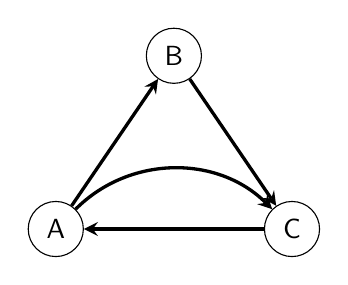
\begin{tikzpicture}[very thick, >=stealth]
			\tikzset{nodo/.style={circle, draw, thin, minimum size=0.7cm, inner sep=0pt, font=\sffamily}}
			
			\node[nodo] (A) at (0, 0) {A};
			\node[nodo] (B) at (1.5, 2.2) {B};
			\node[nodo] (C) at (3, 0) {C};
			
			\draw[->] (A) -- (B);
			\draw[->] (B) -- (C);
			\draw[->] (C) -- (A);
			
			% Curvatura aumentata per distaccare meglio la freccia bidirezionale dal lato del triangolo
			\draw[->, bend left=45] (A) to (C);
		\end{tikzpicture}
	\end{center}
	
	È importante notare che possiamo avere anche due archi sugli stessi nodi ma con orientamento diverso (come mostrato nel collegamento bidirezionale).
	
	\begin{definizione}{Arco incidente e vertici adiacenti}{}
		Sia $f$ un arco che collega due vertici $x$ e $y$, formalmente rappresentabile come $x \longleftarrow f \longrightarrow y$. Diciamo che:
		\begin{itemize}
			\item L'arco $f$ è \textbf{incidente} ai vertici $x$ e $y$.
			\item Il vertice $x$ è \textbf{adiacente} al vertice $y$.
		\end{itemize}
	\end{definizione}
	
	\begin{definizione}{Grado di un vertice}{}
		Il \textbf{grado} di un vertice $x$, denotato con $\deg(x)$, è dato dal numero di archi incidenti in $x$.
	\end{definizione}
	
	Ad esempio, considerando un nodo centrale collegato a quattro vertici periferici:
	
	\begin{center}
		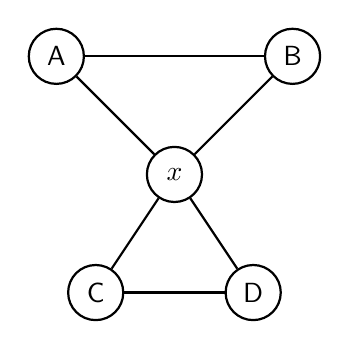
\begin{tikzpicture}[thick]
			\tikzset{nodo/.style={circle, draw, minimum size=0.7cm, inner sep=0pt, font=\sffamily}}
			
			% Nodo centrale (evidenziato con la x come da testo)
			\node[nodo] (X) at (1.5, 1.5) {$x$};
			
			% Nodi periferici
			\node[nodo] (A) at (0, 3) {A};
			\node[nodo] (B) at (3, 3) {B};
			\node[nodo] (C) at (0.5, 0) {C};
			\node[nodo] (D) at (2.5, 0) {D};
			
			\draw (X) -- (A);
			\draw (X) -- (B);
			\draw (X) -- (C);
			\draw (X) -- (D);
			
			% Collegamenti esterni
			\draw (A) -- (B);
			\draw (C) -- (D);
		\end{tikzpicture}
	\end{center}
	
	Per il nodo centrale $x$ contrassegnato, avremo chiaramente $\deg(x) = 4$, poiché vi incidono esattamente quattro archi \textbf{distinti}.
	
	\section{Il problema dei ponti di Konigsberg}
	
	Il problema classico da cui nasce la teoria dei grafi è il famoso problema dei ponti di Konigsberg:
	\begin{figure}[htbp]
		\centering
		\includegraphics[width=0.5\textwidth]{konigsberg_bridges_problem.png}
		\caption{Rappresentazione grafica del problema dei ponti di Konigsberg.}
	\end{figure}
	
	Ci si chiede: \textit{è possibile attraversare tutti i ponti una sola volta e tornare al punto di partenza?}
	Come prima cosa, quando si vuole tradurre un problema in un problema di teoria dei grafi, è buona cosa cercare di dare una rappresentazione grafica il più accurata possibile del problema.
	Essendo questo un problema di piccole dimensioni, possiamo ottenere la seguente struttura:
	\begin{figure}[htbp]
		\centering
		\includegraphics[width=0.5\textwidth]{konigsberg_graph.png}
		\caption{Rappresentazione a grafo del problema dei ponti.}
	\end{figure}
	
	Si invita il lettore a provare manualmente se esiste tale sequenza di attraversamenti, ma la risposta alla domanda rimane \textbf{negativa}.
	Prima di giustificarne la motivazione, dobbiamo fornire delle importantissime definizioni riguardanti i grafi.
	
	\begin{definizione}{Passeggiata in un grafo}{}
		Una \textbf{passeggiata} (o \textbf{walk}) in un grafo è una sequenza $v_0, e_1, v_1, e_2, v_2, \dots, v_{k-1}, e_k, v_k$ che alterna vertici e archi.
		Formalmente, può essere anche indicata con $W = (v_1, v_2, \dots, v_k)$, dunque omettendo gli archi ma indicando solo in ordine di apparizione i vertici.
	\end{definizione}
	
	\begin{definizione}{Passeggiata chiusa}{}
		Una passeggiata si dice \textbf{chiusa} se $v_0 = v_k$, cioè il punto di inizio coincide con il punto di arrivo.
	\end{definizione}
	
	Possiamo adesso giustificare, più o meno, la risposta al problema dei ponti di Konigsberg: qualsiasi grafo con almeno un nodo $x$ con grado dispari \textbf{non} ammette una passeggiata chiusa che utilizza tutti gli archi una sola volta.
	
	E se invece tutti i nodi avessero grado pari? Interessante, domanda, ma \textbf{non è detto}.
	
	\begin{figure}[htbp]
		\noindent\begin{minipage}[c]{0.50\textwidth}
			\centering
			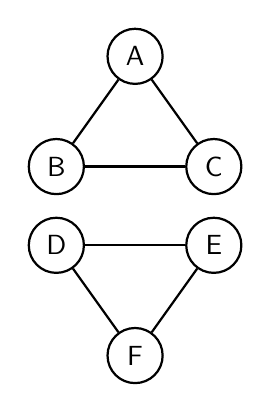
\begin{tikzpicture}[thick, baseline=(current bounding box.center)]
				% Stile coerente con i grafi precedenti
				\tikzset{nodo/.style={circle, draw, minimum size=0.7cm, inner sep=0pt, font=\sffamily}}
				
				% Triangolo superiore (vertice in alto)
				\node[nodo] (A) at (1, 3.2) {A};
				\node[nodo] (B) at (0, 1.8) {B};
				\node[nodo] (C) at (2, 1.8) {C};
				
				\draw (A) -- (B);
				\draw (B) -- (C);
				\draw (C) -- (A);
				
				% Triangolo inferiore (vertice in basso, non connesso al primo)
				\node[nodo] (D) at (0, 0.8) {D};
				\node[nodo] (E) at (2, 0.8) {E};
				\node[nodo] (F) at (1, -0.6) {F};
				
				\draw (D) -- (E);
				\draw (E) -- (F);
				\draw (F) -- (D);
				
			\end{tikzpicture}
		\end{minipage}\hfill%
		\begin{minipage}[c]{0.45\textwidth}
			\caption{Grafo non connesso formato da due componenti triangolari disgiunte. Tutti i vertici hanno $\deg(v) = 2$, ma il grafo complessivo non è connesso e dunque non è possibile effettuare una passeggiata chiusa al suo interno.}
		\end{minipage}
	\end{figure}
	
	\begin{definizione}{Grafo connesso}{}
		Un grafo si dice \textbf{connesso} se per ogni coppia di vertici esiste una passeggiata da $x$ a $y$.
		In poche parole, un grafo si dice connesso se ogni coppia di vertici scelta è collegata in qualche modo.
	\end{definizione}
	
	\begin{teorema}{Caratterizzazione di Eulero}{}
		Esiste una passeggiata chiusa che contiene ogni arco una sola volta se e solo se:
		\begin{enumerate}
			\item Ogni vertice ha \textbf{grado pari}.
			\item Il grafo è \textbf{connesso}.
		\end{enumerate}
	\end{teorema}
	
	\newpage
	\section{Rappresentazione fisica dei grafi}
	
	La rappresentazione informatica dei grafi in memoria è fondamentale per determinare l'efficienza degli algoritmi che operano su di essi. Esistono principalmente due modalità standard per rappresentare un grafo: le \textbf{matrici di adiacenza} e le \textbf{liste di adiacenza}.
	
	\subsection{Matrici di adiacenza}
	Si stabilisce una matrice $n \times n$ dove $n = \#V$, e dove:
	\[
	m_{i,j} = \begin{cases}
		1 & \text{se } i \text{ è adiacente a } j \\
		0 & \text{altrimenti}
	\end{cases}
	\]
	
	\textbf{Esempio:}
	\begin{center}
		\begin{minipage}{0.45\textwidth}
			\centering
			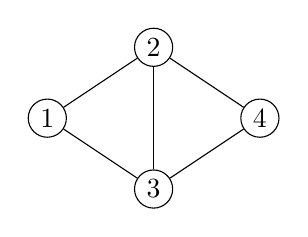
\begin{tikzpicture}[scale=0.9, every node/.style={circle,draw,inner sep=2pt}]
				\node (1) at (0,1) {$1$};
				\node (2) at (1.5,2) {$2$};
				\node (3) at (1.5,0) {$3$};
				\node (4) at (3,1) {$4$};
				
				\draw (1) -- (2);
				\draw (1) -- (3);
				\draw (2) -- (3);
				\draw (2) -- (4);
				\draw (3) -- (4);
			\end{tikzpicture}
		\end{minipage}
		\begin{minipage}{0.45\textwidth}
			\centering
			\[
			\begin{matrix}
				& \begin{matrix} 1 & 2 & 3 & 4 \end{matrix} \\
				\begin{matrix} 1 \\ 2 \\ 3 \\ 4 \end{matrix} &
				\begin{bmatrix}
					0 & 1 & 1 & 0 \\
					1 & 0 & 1 & 1 \\
					1 & 1 & 0 & 1 \\
					0 & 1 & 1 & 0
				\end{bmatrix}
			\end{matrix}
			\]
		\end{minipage}
	\end{center}
	
	Se il grafo non è diretto, la matrice sarà simmetrica rispetto alla diagonale.
	
	Vediamo di seguito il \textbf{costo computazionale} di alcune delle operazioni elementari che possono essere effettuate sui grafi:
	\begin{itemize}
		\item \textbf{Visita del grafo e memorizzazione}: $\mathbf{\Theta(n^2)}$, in quanto viene memorizzato come una matrice $n \times n$.
		
		\item Per verificare se $\mathbf{i}$ \textbf{è adiacente a} $\mathbf{j}$: $\mathbf{\Theta(1)}$, in quanto è sufficiente controllare il valore di $M[i][j]$: se esso corrisponde ad 1 allora i due nodi sono adiacenti, altrimenti no.
		
		\item \textbf{Verificare il grado di un dato vertice} $\mathbf{i}$: $\mathbf{\Theta(n)}$, in quanto occorre scorrere la riga $i$-esima della matrice e contare quanti $1$ ci sono.
	\end{itemize}
	
	\newpage
	\subsection{Liste di adiacenza}
	
	Una lista di adiacenza è composta da:
	\begin{itemize}
		\item Un array in cui ogni elemento è un nodo del grafo.
		
		\item Per ogni nodo del grafo, dunque per ogni elemento dell'array, viene associato anche un puntatore \texttt{neigbh} che punta ad una lista concatenata contenente tutti i nodi adiacenti al nodo corrente.
	\end{itemize}
	
	\begin{figure}[htbp]
		\noindent\begin{minipage}[c]{0.48\textwidth}
			\centering
			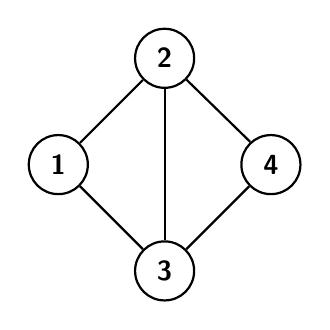
\begin{tikzpicture}[thick, scale=0.9, baseline=(current bounding box.center)]
				% Stile per i nodi del grafo
				\tikzset{nodo/.style={circle, draw, minimum size=0.75cm, inner sep=0pt, font=\bfseries\sffamily}}
				
				% Posizionamento nodi (disposizione a rombo/aquilone)
				\node[nodo] (1) at (0, 1.5) {1};
				\node[nodo] (2) at (1.5, 3) {2};
				\node[nodo] (3) at (1.5, 0) {3};
				\node[nodo] (4) at (3, 1.5) {4};
				
				% Archi definiti dalla lista di adiacenza
				\draw (1) -- (2);
				\draw (1) -- (3);
				\draw (2) -- (3);
				\draw (2) -- (4);
				\draw (3) -- (4);
			\end{tikzpicture}
		\end{minipage}\hfill%
		\begin{minipage}[c]{0.48\textwidth}
			\centering
			% Rappresentazione formale della lista di adiacenza
			$\begin{bmatrix}
				1 \\
				2 \\
				3 \\
				4
			\end{bmatrix}
			\begin{array}{l}
				\longrightarrow [2, 3] \\[4pt]
				\longrightarrow [1, 3, 4] \\[4pt]
				\longrightarrow [1, 2, 4] \\[4pt]
				\longrightarrow [2, 3]
			\end{array}$
		\end{minipage}
	\end{figure}
	
	\textbf{Costo computazionale} delle operazioni elementari:
	\begin{itemize}
		\item Per visitare e memorizzare: $\mathcal{O}\left(n + \sum_{v} \deg(v)\right) = \mathcal{O}(n + 2m) = \mathcal{O}(n + m)$.\\
		Spieghiamo il perché di questo costo computazionale:
		\begin{enumerate}
			\item Sicuramente, per memorizzare una lista di adiacenza abbiamo bisogno innanzitutto di un array che tenga traccia di tutti i nodi. Ecco da dove viene il $\mathcal{O}(n)$.
			
			\item Inoltre, per ogni nodo dobbiamo memorizzare anche tutti i nodi a lui adiacenti. Il numero di nodi adiacenti corrisponde al \textbf{grado} del singolo nodo, ossia al numero di archi incidenti al nodo. Sappiamo che il numero di archi è quantificabile con $m$, ma in questo caso stiamo contando ogni arco ben due volte (vedendo anche l'esempio, nel nodo 1 stiamo dicendo che è adiacente a 2, e nel nodo due stiamo dicendo che è adiacente ad 1). Dovremo dunque contare due volte ogni arco, ottenendo una quantità pari a $2m$. Il costo computazionale diventa dunque nell'ordine di $n + 2m$, ma sapendo che le costanti moltiplicative sono indifferenti asintoticamente, tale valore diventa semplicemente $O(n + m)$.
		\end{enumerate}
		
		\item Per verificare se $i$ è adiacente a $j$: $\mathcal{O}(\deg(i))$. Questo in quanto come vediamo la lista di adiacenza relativa ad ogni nodo ha un numero di elementi pari al grado di quel nodo. Dunque per verificare se due nodi sono adiacenti o meno è necessario scorrere la lista di adiacenza di quel nodo e cercare il nodo adiacente interessato.
	\end{itemize}
	
	Per quanto riguarda la memorizzazione e la visita completa di un grafo memorizzato mediante liste di adiacenza, si potrebbe fare un appunto riguardo ai grafi diretti. In tal caso, a meno che ogni arco non sia bi-direzionale, verrebbe memorizzata letteralmente \textbf{la metà} dei nodi memorizzati in un grafo non orientato.
	\begin{osservazione}{}{}
		Supponiamo di avere un problema che ci richieda frequentemente quali nodi puntano verso un dato nodo $u$.
		Se mantenessimo un'implementazione mediante liste di adiacenza come quella vista in figura, per trovare tutti i nodi collegati ad $u$ dovremmo scorrere per ogni nodo nella lista le sue liste di adiacenza, ottenendo un costo computazionale di $\mathcal{O}(n + m)$, come se fosse una normale visita.\\
		\smallbreak
		Se invece decidessimo di modificare leggermente la struttura della lista di adiacenza, aggiungendo per ogni nodo un puntatore ai suoi nodi entranti e uscenti, il costo computazionale di tale operazione si ridurrebbe ad un misero $\mathcal{O}(\operatorname{deg}(u))$, in quando dovremo scorrere solo la lista dei nodi entranti (il cui numero corrisponde appunto al grado del nodo).
		Nota bene che questa implementazione non appesantisce così tanto il costo di memorizzazione della struttura dati, in quanto per ogni nodo $u$ si aggiunge $\mathcal{O}(\operatorname{deg}(u))$ di costo computazionale, portando il totale ad $\mathcal{O}(n+3m = \mathcal{O}(n+m))$.
	\end{osservazione}
	
	\section{Passeggiate e cammini}
	
	\begin{definizione}{Cammino}{}
		Un \textbf{cammino} nel grafo è una passeggiata in cui non viene ripetuto alcun vertice.
	\end{definizione}
	
	\begin{figure}[htbp]
		\noindent\begin{minipage}[c]{0.50\textwidth}
			\centering
			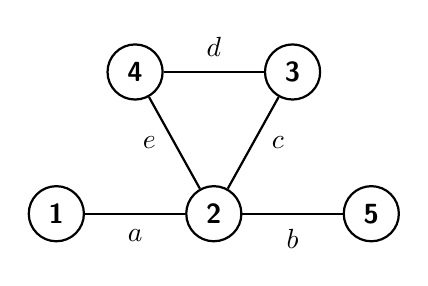
\begin{tikzpicture}[thick, baseline=(current bounding box.center)]
				% Stile per i nodi del grafo
				\tikzset{nodo/.style={circle, draw, minimum size=0.7cm, inner sep=0pt, font=\sffamily\bfseries}}
				
				% Nodi
				\node[nodo] (1) at (0, 0) {1};
				\node[nodo] (2) at (2, 0) {2};
				\node[nodo] (5) at (4, 0) {5};
				\node[nodo] (4) at (1, 1.8) {4};
				\node[nodo] (3) at (3, 1.8) {3};
				
				% Archi con relative etichette (lettere minuscole)
				\draw (1) -- (2) node[midway, below=2pt] {$a$};
				\draw (2) -- (5) node[midway, below=2pt] {$b$};
				\draw (2) -- (3) node[midway, right=3pt] {$c$};
				\draw (4) -- (3) node[midway, above=2pt] {$d$};
				\draw (4) -- (2) node[midway, left=3pt] {$e$};
			\end{tikzpicture}
		\end{minipage}\hfill%
		\begin{minipage}[c]{0.45\textwidth}
			\caption{Una passeggiata potrebbe essere: $1\ a\ 2\ c\ 3\ d\ 4\ e\ 2\ b\ 5$.\\
			Una camminata da $1$ a $5$ potrebbe invece essere $1\ a \ 2\ b\ 5$.}
			\label{fig:passeggiata_grafo}
		\end{minipage}
	\end{figure}
	
	\begin{corollario}{}{}
		Esiste una passeggiata da $x$ a $y$ $\iff$ esiste un cammino da $x$ a $y$.
	\end{corollario}
	
	\begin{dimostrazione}{}{}
		Chiaramente, se esiste un cammino allora sicuramente esiste anche una passeggiata, dato che ogni cammino è un particolare tipo di passeggiata. Abbiamo così dimostrato la prima implicazione ($\Rightarrow$).\\
		\smallbreak
		Viceversa, supponiamo di avere una passeggiata $W = (v_0, v_1, \dots, v_K)$. Abbiamo due possibilità:
		\begin{enumerate}
			\item Se tutti i vertici sono distinti, allora la passeggiata è già un cammino.
			\item Se invece abbiamo almeno un indice ripetuto, cioè esistono $i, j$ tali che $v_i = v_j$ con $i < j$.
		\end{enumerate}
		Questo significa che all'interno della passeggiata è presente un sottociclo:
		\[
		W_1 = (v_i, v_{i+1}, \dots, v_{j-1}, v_j)
		\]
		ma sapendo che $v_i = v_j$, la struttura si chiude. Possiamo eliminare $W_1$ dalla passeggiata iniziale mantenendo però il nodo in cui parte la diramazione (in questo caso $v_i$). La passeggiata iniziale può essere dunque riscritta come:
		\[
		W = (v_1, \dots, v_i, \underbrace{v_{i+1}, \dots, v_{j-1}, v_j}_{W_1}, v_{j+1}, \dots, v_K)
		\]
		Eliminando $W_1$ otteniamo un cammino più corto, e reiterando il procedimento rimuoviamo tutti i cicli ottenendo infine un cammino semplice.
	\end{dimostrazione}
	
	\begin{definizione}{Ciclo}{}
		Un \textbf{ciclo} è un grafo connesso in cui \textbf{ogni vertice ha grado 2}.
	\end{definizione}
	
	\begin{figure}[htbp]
		\noindent\begin{minipage}[c]{0.50\textwidth}
			\centering
			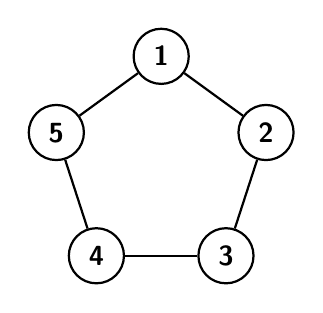
\begin{tikzpicture}[thick, baseline=(current bounding box.center)]
				% Stile dei nodi
				\tikzset{nodo/.style={circle, draw, minimum size=0.7cm, inner sep=0pt, font=\sffamily\bfseries}}
				
				% Raggio del pentagono
				\def\r{1.4cm}
				
				% Nodi disposti in cerchio a intervalli di 72 gradi (partendo dall'alto a 90°)
				\node[nodo] (1) at (90:\r)  {1};
				\node[nodo] (2) at (18:\r)  {2};
				\node[nodo] (3) at (306:\r) {3};
				\node[nodo] (4) at (234:\r) {4};
				\node[nodo] (5) at (162:\r) {5};
				
				% Archi del ciclo
				\draw (1) -- (2);
				\draw (2) -- (3);
				\draw (3) -- (4);
				\draw (4) -- (5);
				\draw (5) -- (1);
			\end{tikzpicture}
		\end{minipage}\hfill%
		\begin{minipage}[c]{0.45\textwidth}
			\caption{Grafo ciclo a 5 vertici ($C_5$).}
			\label{fig:grafo_ciclo_c5}
		\end{minipage}
	\end{figure}
	
	\section{Algoritmo di ricerca di un ciclo all'interno di un grafo}
	
	Proponiamo un altro problema classico del lavoro con i grafi: supponiamo che, dato un grafo $G$ con l'ipotesi che \textbf{ogni vertice ha grado 2 o superiore}, volessimo trovare un qualsiasi ciclo nel grafo.
	Partiamo con un esempio grafico di un grafo che contiene un ciclo, e vediamo come procederemmo umanamente.
	\begin{figure}[htbp]
		\begin{minipage}[c]{1\textwidth}
			\centering
			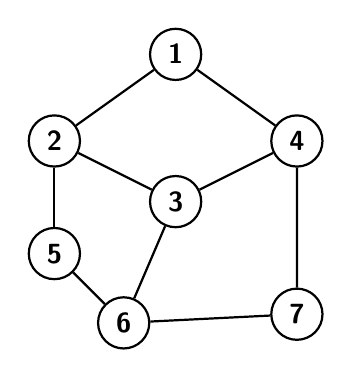
\begin{tikzpicture}[thick, scale=1.1, baseline=(current bounding box.center)]
				% Stile per i vertici
				\tikzset{nodo/.style={circle, draw, minimum size=0.65cm, inner sep=0pt, font=\sffamily\bfseries}}
				
				% Faccia superiore (rombo superiore)
				\node[nodo] (T_back)  at (1.2, 2.7) {1};
				\node[nodo] (T_left)  at (-0.2, 1.7) {2};
				\node[nodo] (T_front) at (1.2, 1.0) {3};
				\node[nodo] (T_right) at (2.6, 1.7) {4};
				
				% Faccia inferiore (traslata in basso)
				\node[nodo] (B_left)  at (-0.2, 0.4) {5};
				\node[nodo] (B_front) at (0.6, -0.4) {6};
				\node[nodo] (B_right) at (2.6, -0.3) {7};
				
				% Vertice nascosto posteriore della base (opzionale per completare la prospettiva isometrica)
				% Nel tuo disegno si vedono i 7 vertici principali con i collegamenti a vista:
				
				% Archi faccia superiore
				\draw (T_back) -- (T_left);
				\draw (T_back) -- (T_right);
				\draw (T_left) -- (T_front);
				\draw (T_right) -- (T_front);
				
				% Archi verticali
				\draw (T_left) -- (B_left);
				\draw (T_front) -- (B_front);
				\draw (T_right) -- (B_right);
				
				% Archi base visibili
				\draw (B_left) -- (B_front);
				\draw (B_front) -- (B_right);
				
			\end{tikzpicture}
		\end{minipage}
	\end{figure}
	
	L'idea di algoritmo chiaramente consiste nel:
	\begin{enumerate}
		\item Scegliere un nodo qualsiasi di partenza.
		
		\item Memorizzarlo all'interno di un apposita struttura dati.
		
		\item Prendere un arco e andare al nodo adiacente. \textbf{Importante} è assicurarsi che il prossimo nodo non sia ancora stato visitato. In tal caso, significa che abbiamo fatto un giro e abbiamo trovato un ciclo.
		
		\item Altrimenti, tornare all'inizio.
	\end{enumerate}
	
	Messa un'idea di base, procediamo con la scrittura dell'effettivo algoritmo in pseudocodice e in seguito alla sua spiegazione.
	
	\begin{lstlisting}[language=Python, caption={Pseudocidice per la ricerca di un ciclo all'interno di un grafo.}]
		def trovaCiclo(G):
			L = lista vuota
			x = un vertice qualsiasi del grafo
			L.append(x)
			
			current = x
			next = x.neigbh[0]
			
			while next not in L:
				L.append(next)
				
				if next.neighbr[0] == current:
					u = next.neighbr[1]
				else:
					u = next.neighbr[0]
					
				current = next
				next = u
				
			while L[0] != next:
				L.remove(0)
				
			return L
	\end{lstlisting}
	
	\begin{algoritmo}{Eestrazione di un ciclo da un grafo}{}
		\begin{enumerate}
			\item Definiamo una lista vuota, per tenere traccia dei nodi visitati finora.
			
			\item Prendiamo un qualsiasi vertice dal quale iniziare la nostra ricerca.
			
			\item Aggiungiamo il nodo scelto all'interno della lista.
			
			\item Prendiamo come prossimo nodo il primo della lista degli adiacenti al nodo corrente.
			
			\item Eseguiamo un ciclo che va avanti finché il next che abbiamo preso non è un nodo già visitato: in tal caso significa che abbiamo intrapreso una strada circolare e siamo tornati indietro.
			
			\item All'interno del ciclo aggiungiamo alla lista \texttt{L} dei nodi visitati anche \texttt{next}.
			
			\item A questo punto dobbiamo scegliere il nuovo \texttt{next}, ma dobbiamo assicurarci che non sia il nodo da cui siamo partiti: ecco perché controlliamo che \texttt{next.neighbr[0]} sia diverso dal nodo su cui siamo adesso, in modo da non poter tornare \textit{subito} indietro.
			
			\item Aggiorniamo i puntatori dei nodi per la prossima iterazione.
			
			\item Una volta usciti da questo ciclo, significa che abbiamo intrapreso la strada circolare di cui si parlava prima, e che dunque abbiamo trovato un ciclo. Significa inoltre che ora il puntatore \texttt{next} punterà al nodo da cui inizia la diramazione del ciclo, e dunque sarà il primo di questo. Ecco perché, nel ciclo finale, controlliamo che \texttt{L[0] != next}, perché \texttt{next} è il primo nodo del ciclo, e dunque deve essere anche il primo della lista che dovremo restituire.
		\end{enumerate}
	\end{algoritmo}
	
	Bisogna fare un appunto su questo algoritmo: ora come ora, per come l'abbiamo scritto, il suo costo computazionale è un $\mathcal{O}(n^2)$, tutto per colpa del controllo di testa del primo ciclo while. La condizione del ciclo è un \texttt{next not in L}, che richiede tempo $\mathcal{O}(n)$ in un array disordinato. Dato che il ciclo while potrebbe poi richiedere fino ad un massimo di $n$ iterazioni, una per ogni nodo del grafo, il costo computazionale sale al tempo quadratico.
	Possiamo ovviamente ottimizzare questo codice, presentando la seguente versione:
	\begin{lstlisting}[language=Python, caption={Ricerca di un ciclo in un grafo ottimizzata}]
		def trovaCiclo(G):
			L = lista vuota
			vis = [0] * n
			
			x = un vertice qualsiasi del grafo
			L.append(x)
			vis[x] = 1
			
			current = x
			next = x.neigbh[0]
			
			while vis[next] == 0:
				L.append(next)
				vis[next] = 1
				
				if next.neighbr[0] == current:
					u = next.neighbr[1]
				else:
					u = next.neighbr[0]
				
				current = next
				next = u
			
			while L[0] != next:
				L.remove(0)
		
		return L
	\end{lstlisting}
	
	\begin{algoritmo}{Ricerca di un ciclo in un grafo}{}
		Andremo a commentare solo le nuove scelte implementative:
		Si è scelto di aggiungere un array \texttt{vis} che verrà usato per tenere traccia degli elementi visitati. Ciò viene fatto stabilendo una biezione tra l'identificativo del nodo e il suo indice all'interno dell'array \texttt{vis}. Così facendo il controllo in testa al ciclo while diventa semplicemente un controllo accedendo ad un elemento dell'array tramite indice, dunque eseguibile in tempo costante.
		L'aggiunta di un array \texttt{vis} che ha una grandezza massima dell'ordine di del numero di nodi $n$ aumenta il costo spaziale da $\Theta(n)$ a $\Theta(n + n) = \Theta(n)$, dunque rimane nello stesso ordine asintotico.
	\end{algoritmo}
	
	Possiamo ora discutere riguardo al costo computazionale dell'algoritmo, per entrambe le versioni:
	\begin{itemize}
		\item Versione inefficiente:
		\begin{itemize}
			\item \textbf{Costo computazionale:} $\mathcal{O}(n^2)$
			\item \textbf{Costo spaziale:} $\Theta(n)$
		\end{itemize}
		
		\item Versione efficiente:
		\begin{itemize}
			\item \textbf{Costo computazionale:} $\Theta(n)$
			\item \textbf{Costo spaziale:} $\Theta(n)$
		\end{itemize}
	\end{itemize}
	
	\section{Visite di un grafo}
	Prima di discutere i modi in cui si possono effettuare le visite su un grafo, diamo alcune definizioni importanti.
	
	\begin{definizione}{Nodo raggiungibile}{}
		Un nodo $y$ si dice \textbf{raggiungibile} da $x$ se $\exists$ un cammino da $x$ a $y$.
	\end{definizione}
	
	\begin{definizione}{Grafo connesso}{}
		Un grafo $G$ si dice \textbf{connesso} se $\forall x, y \in V(G),\, \exists$ un cammino da $x$ a $y$.
	\end{definizione}
	
	Le visite nascono per rispondere alla problematica classica: \textit{Esiste un cammino da $x$ a $y$?}
	
	Il metodo più sicuro consiste nel \textbf{visitare}, a partire dal nodo $x$, uno ad uno tutti i nodi del grafo. Ovviamente, se durante tale visita si incontra il nodo $y$, la risposta alla domanda sarà affermativa.
	
	Ciò si può fare principalmente in due modi:
	
	\begin{description}
		\item [DFS (\textit{Depth-First-Search}, Visita in profondità):] 
		Funziona come l'esplorazione di un labirinto: si sceglie un percorso e si avanza finché non si trova un vicolo cieco. A quel punto si torna indietro fino al primo incrocio in cui si sono lasciate strade inesplorate e si prova un'altra via.
		
		\item [BFS (\textit{Breadth-First-Search}, Visita in ampiezza):] 
		Preso un nodo iniziale, si visitano prima tutti i suoi vicini diretti, poi i vicini dei vicini, e così via.
	\end{description}
	
	\subsection{DFS - Depth-First-Search}
	Vediamo per prima la visita DFS.
	
	In base alla brevissima e introduttiva descrizione dell'algoritmo fornita poco fa, possiamo delinearne un'idea algoritmica di base:
	\begin{enumerate}
		\item Partiamo da un nodo $x$ e lo segniamo come visitato.
		\item Scegliamo una strada inesplorata verso cui procedere.
		\item Segniamo il nodo scelto come visitato e ripetiamo la visita ricorsivamente o iterativamente.
	\end{enumerate}
	
	La modalità di backtracking verrà implementata mediante una pila (\emph{stack}), che lavora secondo il principio LIFO (\emph{Last In, First Out}). Dunque, quando dobbiamo tornare indietro, basta effettuare un'operazione di \texttt{pop()} per tornare al nodo precedentemente esaminato.
	
	Vediamo una prima implementazione iterativa dell'algoritmo:
	
	\begin{lstlisting}[style=stile-listings, language=Python, caption={Implementazione iterativa della DFS}]
		DFS(G, x):
			vis = [0] * n
			S = uno stack
			S.push(x)
			vis[x] = 1
			
			while S.size() != 0:
				y = S.top()
				if esiste un vicino z di y che non è stato visitato (vis[z] == 0):
					S.push(z)
					vis[z] = 1
				else:
					S.pop()
		
			return vis
	\end{lstlisting}
	
	\begin{algoritmo}{Analisi dettagliata dell'algoritmo DFS}{}
		Analizziamo riga per riga il funzionamento dell'implementazione:
		\begin{itemize}
			\item \texttt{vis = [0] * n}: Inizializziamo l'array per tenere traccia dei nodi visitati.
			
			\item \texttt{S = uno stack}: Inizializziamo lo stack per permettere il backtracking.
			
			\item \texttt{S.push(x)} e \texttt{vis[x] = 1}: Aggiungiamo il nodo di partenza allo stack e lo segniamo come visto.
			
			\item \texttt{while S.size() != 0}: Iteriamo finché lo stack non rimane vuoto, il che vorrà dire che ogni nodo raggiungibile è stato esaminato.
			
			\item \texttt{y = S.top()}: Prendiamo il nodo in cima allo stack, che rappresenta il nodo corrente.
			
			\item \textbf{Controllo del vicino}: Se la condizione di entrata è rispettata (esiste un vicino $z$ tale che \texttt{vis[z] == 0}), vuol dire che possiamo continuare per un'altra strada, cioè quella verso $z$. Di conseguenza effettuiamo il \texttt{push} di $z$ e lo marchiamo come visitato.
			
			\item \textbf{Gestione del vicolo cieco (\emph{else})}: Altrimenti, significa che abbiamo raggiunto un ``vicolo cieco'' e che dobbiamo tornare indietro. Nel pratico, questo si traduce nel rimuovere l'elemento in cima alla pila tramite \texttt{S.pop()}, così che alla prossima iterazione i controlli vengano fatti sul nodo da cui siamo arrivati e sui suoi rimanenti vicini.
			
		\end{itemize}
	\end{algoritmo}
	
	Seppur si tratti di un'implementazione molto descrittiva dell'algoritmo, analizziamo il controllo condizionale: dobbiamo prendere il nodo $y$, controllarne i vicini e verificare che almeno per un vicino $z$ valga la condizione \texttt{vis[z] == 0}. 
	
	Questo controllo corrisponde a una ricerca sequenziale che, come ben sappiamo, richiede tempo $O(n)$ nel caso peggiore per singolo nodo, se non opportunamente ottimizzata.
	
	È poi facile verificare come il ciclo \texttt{while} si ripeta tante volte quanti sono i nodi del grafo, dunque $\Theta(n)$.
	
	Combinando queste due osservazioni, otteniamo che il costo di questa versione è $O(n^2)$, che risulta non essere particolarmente ottimale.
	
	\smallbreak
	Proponiamo di seguito una versione ottimizzata dell'algoritmo.	
	\begin{lstlisting}[style=stile-listings, language=Python]
		def DFS_ottimizzato(G, x):
			vis = [0] * len(G)
			vis[x] = 1
			
			s = Stack()
			s.push(x)
			
			while s.size() != 0:
				current = s.pop()
				for v in current.neighbor: # (2)
					if vis[v] == 0:
						vis[v] = 1
						s.push(v)
			
			return vis
	\end{lstlisting}
	
	\begin{algoritmo}{Visita DFS ottimizzata}{dfs_ottimizzata}
		La differenza rispetto alla versione non ottimizzata risiede in due passaggi chiave:
		\begin{enumerate}
			\item In \textbf{(1)} estraiamo il nodo corrente dalla pila. Così facendo lo eliminiamo dalla pila e non dal grafo, evitando modifiche distruttive alla struttura dati; in questo modo il nodo \texttt{current} non verrà mai più controllato nelle iterazioni successive.
			\item In \textbf{(2)} andiamo a verificare ciascun vertice adiacente a quello appena estratto. Se non è ancora stato visitato, lo marchiamo come visitato e lo inseriamo nella pila, così da poter proseguire l'esplorazione a partire da esso.
		\end{enumerate}
	\end{algoritmo}
	
	Questa versione dell'algoritmo presenta la seguente complessità:
	\begin{itemize}
		\item \textbf{Costo spaziale}: $\Theta(n)$, dovuto all'array dei nodi visitati e allo spazio occupato dalla pila nel caso peggiore.
		\item \textbf{Costo temporale}: il ciclo \texttt{while} viene eseguito $n$ volte, esattamente una volta per ciascun vertice. All'interno del ciclo viene eseguito un lavoro costante $\Theta(1)$ per l'operazione di estrazione (\texttt{pop}) e un costo pari a $O(\operatorname{deg}(\text{current}))$ per scorrere l'intera lista di adiacenza del nodo estratto.
	\end{itemize}
	
	Il costo computazionale complessivo del ciclo è quindi descritto dalla seguente sommatoria:
	\begin{align*}
		\sum_{i=1}^n \Big( O(1) + O(\operatorname{deg}(G[i])) \Big)
		&= \sum_{i=1}^n 1 + \sum_{i=1}^n \operatorname{deg}(G[i]) = \\
		&= O(n) + O(2m) = O(n + 2m) = O(n + m)
	\end{align*}
	
	Per completezza, essendo i grafi un soprainsieme degli alberi, scriviamo una versione ricorsiva della DFS divisa in una funzione ausiliaria e nella visita effettiva.
	
	\begin{lstlisting}[language=Python]
		def dfs(G, x):
			vis = [0] * n
			return dfs_ric(G, x, vis)
			
		def dfs_ric(G, x, vis):
			vis[x] = 1
			for v in x.neighbr:
				if vis[v] == 0:
					dfs_ric(G, v, vis)
	\end{lstlisting}
	
	La visita costa sempre $O(n+m)$. L'unica limitazione è lo stack delle funzioni, che per grafi molto pieni potrebbe andare in \textit{recursion depth}.
	
	\begin{dimostrazione}{Correttezza della DFS ricorsiva}{}
		Dimostriamo ora che questo algoritmo funziona.
		
		Appuntiamo che se un nodo $y$ è raggiungibile a partire da $x$, allora esiste un cammino che collega $x \to y$ e dunque $\text{vis}[y] = 1$.
		Se $y$ è raggiungibile da $x \implies \exists W = (v_0, v_1, \dots, v_k)$ cammino che collega $x$ ($v_0$) e $y$ ($v_k$).
		
		Per assurdo, assumiamo che $\text{vis}[y] = 0$.
		Siccome $\text{vis}[x] = 1 \implies \exists$ un indice $i$ con $\text{vis}[v_i] = 1$ e $\text{vis}[v_{i+1}] = 0$.
		Se $\text{vis}[v_i] = 1$ allora $v_i$ è stato visitato ed è stato inserito nello stack $S$.
		Dato che l'algoritmo è terminato, significa che ad un certo punto $v_i$ è stato rimosso dallo stack.
		
		\textbf{Contraddizione}: se è stato rimosso, vuol dire che tutti gli adiacenti a $v_i$ erano a loro volta stati visitati. Tuttavia prima avevamo detto che $\text{vis}[v_{i+1}] = 0$, dunque abbiamo dimostrato per assurdo che l'algoritmo funziona.
	\end{dimostrazione}
	
	Proponiamo ora un esercizio che ci aiuterà a lavorare con i grafi e con la visita in profondità (DFS).
	
	\begin{esercizio}{Calcolo delle componenti connesse tramite DFS}{}
		Modificare l'algoritmo di visita DFS al fine di calcolare $\text{num\_comp}$, ovvero il numero totale di componenti connesse di un grafo, e popolare un array $\text{comp}[]$ con valori appartenenti a $\{1, \dots, \text{num\_comp}\}$ tale che:
		\[
		\text{comp}[x] = \text{comp}[y] \iff x \text{ e } y \text{ appartengono alla stessa componente connessa}
		\]
	\end{esercizio}
	
	\paragraph{Esempio.}
	Consideriamo il seguente grafo disconnesso formato da due componenti connesse:
	
	\begin{center}
		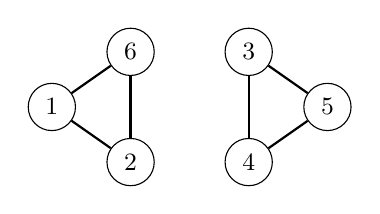
\begin{tikzpicture}[scale=1.0, every node/.style={circle, draw, font=\small, inner sep=2pt, minimum size=6mm}]
			% Componente 1
			\node (1) at (0, 0.5) {1};
			\node (6) at (1, 1.2) {6};
			\node (2) at (1, -0.2) {2};
			
			\draw[thick] (1) -- (6);
			\draw[thick] (6) -- (2);
			\draw[thick] (2) -- (1);
			
			% Componente 2
			\node (3) at (2.5, 1.2) {3};
			\node (4) at (2.5, -0.2) {4};
			\node (5) at (3.5, 0.5) {5};
			
			\draw[thick] (3) -- (5);
			\draw[thick] (5) -- (4);
			\draw[thick] (4) -- (3);
		\end{tikzpicture}
	\end{center}
	
	In questo caso il risultato dell'algoritmo sarà:
	\[
	\text{num\_comp} = 2, \qquad \text{comp} = [1, 1, 2, 2, 2, 1]
	\]
	dove la posizione $i$-esima dell'array $\text{comp}$ indica la componente di appartenenza del nodo $i$.
	
	Diamo prima un'idea generale della struttura dell'algoritmo:	
	\begin{enumerate}
		\item \textbf{Inizializzazione delle strutture dati globali}:
		Inizializziamo l'array globale $\text{comp}$ di dimensione $n$ impostando tutti i valori a $0$. Impostiamo inoltre la variabile globale $\text{num\_comp} = 0$.
		
		\item \textbf{Avvio della DFS}:
		Selezioniamo il primo nodo non ancora visitato, incrementiamo il contatore ($\text{num\_comp} = \text{num\_comp} + 1$) ed eseguiamo la DFS a partire da esso.
		
		\item \textbf{Assegnazione della componente durante la DFS}:
		All'interno della funzione DFS, per ogni vertice $v$ raggiunto durante la visita, impostiamo:
		\[
		\text{comp}[v] = \text{num\_comp}
		\]
		L'utilità dell'array \texttt{comp} sta anche nel fatto che può benissimo rimpiazzare l'array \texttt{vis} che avevamo precedentemente usato per marcare i nodi visitati. Avendolo inizializzato con tutti 0, i nodi non ancora visitati avranno \texttt{comp[v] = 0}.
		
		\item \textbf{Scorrimento di tutti i vertici}:
		Terminata la singola DFS, si prosegue scorrendo l'elenco dei vertici del grafo:
		\begin{itemize}
			\item Se \texttt{comp[v] != 0}, il nodo è già stato visitato e possiamo passare al successivo.
			\item Altrimenti, incrementiamo \texttt{num\_comp = num\_comp +1} e riavviamo la DFS dal nodo $v$.
		\end{itemize}
	\end{enumerate}
	
	Avendo discusso l'idea dell'algoritmo, possiamo fornirne un esempio di implementazione
	\begin{lstlisting}[style=stile-listings, language=Python]
		trova_comp(G):
			comp = [0] * n
			num_comp = 0
			S = Stack()
			
			for v in G:
				if comp[v] == 0:
					num_comp += 1
					S.push(v)
					comp[v] = num_comp
			
					while S.size() != 0:
						current = S.pop()
						for w in current.neighbor:
							if comp[w] == 0:
								comp[w] = num_comp
								S.push(w)
			
			return comp, num_comp
	\end{lstlisting}
	
	\begin{algoritmo}{Algoritmo per la ricerca delle componenti connesse}{alg_trova_comp}		
		\begin{itemize}
			\item \textbf{Inizializzazione}: Viene creato un vettore \texttt{comp} di dimensione $n$ inizializzato a $0$, che servirà anche a segnalare i nodi visitati, un contatore \texttt{num\_comp} impostato a $0$ e una struttura dati di tipo \texttt{Stack}.
			
			\item \textbf{Identificazione di una nuova componente}: Nel ciclo \texttt{for v in G}, l'istruzione \texttt{if comp[v] == 0} verifica se il nodo $v$ non è ancora stato visitato. Se questa condizione è vera, significa che ci troviamo su una \textbf{nuova componente connessa}, in quanto il nodo corrente non appartiene a nessuna componente precedentemente esplorata.
			
			\item \textbf{Assegnazione ed esplorazione}:
			\begin{enumerate}
				\item Si incrementa il contatore delle componenti (\texttt{num\_comp += 1}).
				\item Si inserisce il nodo sorgente $v$ nello stack \texttt{S} e se ne assegna l'indice della componente corrispondente (\texttt{comp[v] = num\_comp}).
				\item Tramite il ciclo \texttt{while S.size() != 0}, si procede all'estrazione di ogni nodo (\texttt{current = S.pop()}) ed all'analisi dei suoi vicini (\texttt{for w in current.neighbor}). Per ciascun vicino non ancora visitato (\texttt{comp[w] == 0}), viene registrata l'appartenenza alla componente corrente e il nodo viene inserito nello stack per ulteriori esplorazioni.
			\end{enumerate}
		\end{itemize}
		
	\end{algoritmo}
	
	Il costo computazionale dell'algoritmo è lo stesso di una normale DFS, dunque risulta essere $\mathcal{O}(n+m)$. Si potrebbe pensare che la DFS venga eseguita una volta per ogni nodo, ma per come abbiamo segnalato i nodi visitati, l'esplorazione viene eseguita \textbf{una sola volta per ogni componente connessa}.
	
	\newpage
	\section{Generici problemi su grafi}
	Prima di continuare il discorso sulle visite, vediamo alcuni esempi di operazioni sui grafi diretti (o orientati).
	\begin{definizione}{Albero di ricerca}{def_albero_ricerca}
		Dati due nodi $x$ e $y$, gli archi che utilizziamo per raggiungere $y$ a partire da $x$ formano il cosiddetto \textbf{albero di ricerca}. 
		
		Si ricorda che un albero è definito come un \textbf{grafo connesso e aciclico}.
	\end{definizione}
	
	\begin{center}
		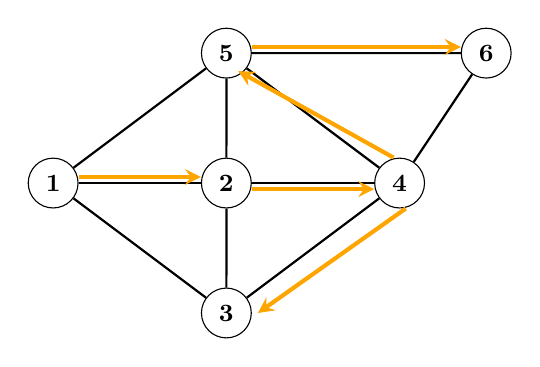
\begin{tikzpicture}[scale=1.1, >=stealth]
			% Stili dei nodi e degli archi
			\tikzstyle{nodo} = [circle, draw=black, fill=white, inner sep=0pt, minimum size=18pt, font=\small\bfseries]
			\tikzstyle{arco} = [line width=0.8pt, black]
			\tikzstyle{albero} = [->, line width=1.5pt, Orange]
			
			% Posizionamento nodi
			\node[nodo] (1) at (0,0) {1};
			\node[nodo] (2) at (2,0) {2};
			\node[nodo] (3) at (2,-1.5) {3};
			\node[nodo] (5) at (2,1.5) {5};
			\node[nodo] (4) at (4,0) {4};
			\node[nodo] (6) at (5,1.5) {6};
			
			% Archi del grafo originale (in nero)
			\draw[arco] (1) -- (5);
			\draw[arco] (1) -- (2);
			\draw[arco] (1) -- (3);
			\draw[arco] (5) -- (2);
			\draw[arco] (2) -- (3);
			\draw[arco] (5) -- (4);
			\draw[arco] (2) -- (4);
			\draw[arco] (3) -- (4);
			\draw[arco] (5) -- (6);
			\draw[arco] (4) -- (6);
			
			% Archi dell'albero di ricerca (in arancione orientato)
			\draw[albero] ([yshift=2pt]1.east) -- ([yshift=2pt]2.west);
			\draw[albero] ([yshift=-2pt]2.east) -- ([yshift=-2pt]4.west);
			\draw[albero] ([xshift=2pt]4.south) -- ([xshift=2pt]3.east);
			\draw[albero] ([xshift=-2pt]4.north) -- ([xshift=-2pt]5.south east);
			\draw[albero] ([yshift=2pt]5.east) -- ([yshift=2pt]6.west);
		\end{tikzpicture}
	\end{center}
	
	Tale albero viene memorizzato mediante il cosiddetto \textbf{"vettore dei padri"}, ovvero un array in cui, per ogni indice $i$, memorizziamo la provenienza dell'esplorazione.
	
	Nell'esempio precedente, il vettore dei padri è rappresentato da:
	\[
	P = \begin{bmatrix}
		\overset{1}{1}, & \overset{2}{1}, & \overset{3}{4}, & \overset{4}{2}, & \overset{5}{4}, & \overset{6}{5}
	\end{bmatrix}
	\]
	in cui, per ogni elemento ad indice $i$, è specificato da quale nodo proviene $i$.
	
	Il nodo radice dell'albero si trova identificando quell'elemento in cui $P[i] == i$, cioè il valore del nodo è uguale al suo indice nell'array.
	
	\begin{esercizio}{Distanza di un nodo dalla radice}{}
		Dato un vettore dei padri $P$ e un vertice $x$, vogliamo trovare la distanza di $x$ dalla radice dell'albero.
	\end{esercizio}
	
	\begin{lstlisting}[language=Python, caption={Risoluzione iterativa}]
		def distRad(P, x):
			count = 0
			while P[x] != x:
				x = P[x]
				count += 1
			return count
	\end{lstlisting}
	
	\begin{lstlisting}[language=Python, caption={Risoluzione ricorsiva}]
		def distRad(P, x):
			if P[x] == x:
				return 0
			return 1 + distRad(P, P[x])
	\end{lstlisting}
	
	Questo algoritmo potrà essere utilizzato in futuro nel corso.
	
	Avendo definito il vettore dei padri, possiamo implementare la visita in profondità (DFS) sfruttando tale struttura. In questa implementazione, il vettore dei padri $P$ viene inizializzato con valori \texttt{null} per indicare i vertici non ancora visitati.
	
	\begin{lstlisting}[style=stile-listings, caption={Algoritmo DFS con vettore dei padri}]
		def dfs_ric(G, x, P):
			for v in x.neighbor:
				if P[v] == null:
					P[v] = x
					dfs_ric(G, v, P)
				
		def dfs(G, x):
			P = [null] * n
			P[x] = x
			dfs_ric(G, x, P)
			return P
	\end{lstlisting}
	
	\subsection{Problema di bicolorazione di un grafo}
	Consideriamo un insieme di $n$ corsi e $m$ studenti. Vogliamo programmare gli esami in due settimane, cioè in modo tale che due esami differenti non possano essere collocati nella stessa settimana. 
	
	Supponiamo che ciascuno studente debba sostenere esattamente due corsi. Questa assunzione è motivata dal fatto che, se uno studente avesse un numero di corsi superiore a tre, sarebbe impossibile evitare di posizionarne almeno due nella stessa settimana.
	\smallbreak
	E' molto importante che, nella risoluzione di un problema di grafi, sappiamo individuare quale dato nel problema corrisponde ai nodi e quale agli archi.
	
	Nel nostro caso, consideriamo un esempio con 4 corsi e 4 studenti, dove ogni studente è associato a una coppia di corsi da frequentare e superare:
	
	\begin{itemize}
		\item Corso $1$: studenti $\{1, 2\}$
		\item Corso $2$: studenti $\{2, 3\}$
		\item Corso $3$: studenti $\{3, 4\}$
		\item Corso $4$: studenti $\{1, 3\}$
	\end{itemize}
	
	Come possiamo osservare, siccome ogni studente è una coppia di esami, questa corrisponde esattamente alla definizione di arco in un grafo. Dunque il grafo $G = (\text{Corsi}, \text{studenti})$ risultante per questo esempio è rappresentato di seguito:
	
	\begin{center}
		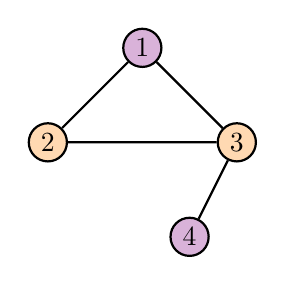
\begin{tikzpicture}[scale=1.2, every node/.style={circle, draw, thick, inner sep=2pt}]
			\node[fill=violet!30] (1) at (1, 2) {$1$};
			\node[fill=orange!30] (2) at (0, 1) {$2$};
			\node[fill=orange!30] (3) at (2, 1) {$3$};
			\node[fill=violet!30] (4) at (1.5, 0) {$4$};
			
			\draw[thick] (1) -- (2);
			\draw[thick] (1) -- (3);
			\draw[thick] (2) -- (3);
			\draw[thick] (3) -- (4);
		\end{tikzpicture}
	\end{center}
	
	Dove i colori dei nodi indicano la settimana assegnata all'esame:
	\begin{itemize}
		\item[$\color{violet}\blacksquare$] Settimana $1$
		\item[$\color{orange}\blacksquare$] Settimana $2$
	\end{itemize}
	
	Come possiamo notare, nell'esempio fornito non è possibile soddisfare il requisito desiderato senza violare i vincoli, poiché i vertici $1$, $2$ e $3$ formano un triangolo (un ciclo di lunghezza dispari).
	
	Il problema della programmazione degli esami in due settimane si riconduce al classico \textbf{problema di bi-colorazione dei grafi}, ovvero determinare se è possibile assegnare uno di due colori (le due settimane) a ciascun vertice in modo tale che ogni arco congiunga due vertici di colore diverso.
	
	\begin{center}
		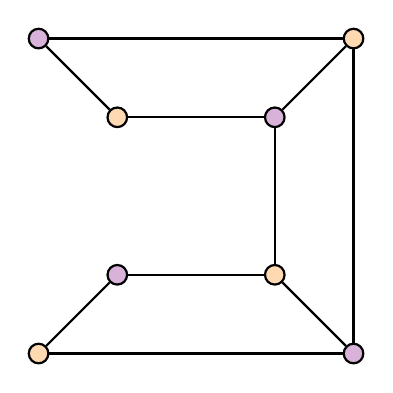
\begin{tikzpicture}[scale=1]
			% Vertici del ciclo esterno
			\node[circle, draw, thick, fill=violet!30, inner sep=2.5pt] (o1) at (-2, 2) {};
			\node[circle, draw, thick, fill=orange!30, inner sep=2.5pt] (o2) at (2, 2) {};
			\node[circle, draw, thick, fill=violet!30, inner sep=2.5pt] (o3) at (2, -2) {};
			\node[circle, draw, thick, fill=orange!30, inner sep=2.5pt] (o4) at (-2, -2) {};
			
			% Vertici del ciclo interno
			\node[circle, draw, thick, fill=orange!30, inner sep=2.5pt] (i1) at (-1, 1) {};
			\node[circle, draw, thick, fill=violet!30, inner sep=2.5pt] (i2) at (1, 1) {};
			\node[circle, draw, thick, fill=orange!30, inner sep=2.5pt] (i3) at (1, -1) {};
			\node[circle, draw, thick, fill=violet!30, inner sep=2.5pt] (i4) at (-1, -1) {};
			
			% Ciclo esterno
			\draw[thick] (o1) -- (o2) -- (o3) -- (o4) -- cycle;
			
			% Ciclo interno
			\draw[thick] (i1) -- (i2) -- (i3) -- (i4) -- cycle;
			
			% Archi tra ciclo esterno e interno
			\draw[thick] (o1) -- (i1);
			\draw[thick] (o2) -- (i2);
			\draw[thick] (o3) -- (i3);
			\draw[thick] (o4) -- (i4);
		\end{tikzpicture}
	\end{center}
	
	\begin{proposizione}{Impossibilità della bi-colorazione}{}
		Il problema di bi-colorazione \textbf{non ha soluzione} per i grafi che contengono \textbf{cicli di lunghezza dispari}.
	\end{proposizione}
	
	L'intuizione dietro questa proprietà è che, percorrendo un ciclo di lunghezza dispari alternando i colori, dovendo assegnare colori diversi a vertici adiacenti, si arriverà inevitabilmente a un punto in cui due vertici adiacenti richiederanno lo stesso colore, rendendo impossibile una colorazione valida.
	
	Quando poniamo un nodo ad un gruppo (ad esempio $1$), allora tutti i suoi adiacenti dovranno appartenere all'altro gruppo ($2$) e viceversa.
	
	Vediamo l'effettivo codice che, preso in input un grafo, restituisce un Array \texttt{part} rappresentante la partizione. Se l'Array restituito risulta essere vuoto, significa che tale grafo non era bi-colorabile.
	
	\begin{lstlisting}[style=stile-listings, language=Python]
		def dfs_part(G, x):
			part = [0] * n
			part[x] = 1
			s = stack()
			s.push(x)
			
			while s.size() != 0:
				y = s.top()
				for v in y.neighbr:
					if part[v] == 0:
						part[v] = 3 - part[y]
						s.push(v)
					else:
						if part[v] == part[y]:
							return []
			return part
	\end{lstlisting}
	
	\begin{algoritmo}{Spiegazione dell'algoritmo di partizione}{}
		Il codice sfrutta una visita in profondità (DFS) modificata per verificare se un grafo ammette una partizione (ad esempio se è bipartito).
		\begin{itemize}
			\item L'array \texttt{part} tiene traccia dello stato di colorazione di ciascun nodo: $0$ indica non visitato/non colorato, mentre $1$ e $2$ rappresentano le due classi di partizione.
			\item Per ogni adiacente $v$ del nodo corrente $y$:
			\begin{enumerate}
				\item Se $v$ non è stato ancora visitato (`part[v] == 0`), gli viene assegnato il colore opposto rispetto a $y$ tramite la formula $3 - \text{part}[y]$, e viene aggiunto allo stack per la visita.
				
				\item Se $v$ è già stato visitato, si controlla che non abbia lo stesso colore del nodo corrente $y$. In caso di conflitto (\texttt{part[v] == part[y]}), il grafo non può essere partizionato e l'algoritmo termina restituendo una partizione vuota.
			\end{enumerate}
		\end{itemize}
		
	\end{algoritmo}
	
	\section{Lavoro su grafi orientati}
	
	In un grafo orientato, la visita DFS funziona ugualmente, ma bisogna prestare attenzione all'orientamento degli archi. Tuttavia nel pratico non cambia nulla, in quanto nella lista di adiacenza di un nodo saranno presenti solo i riferimenti ai nodi che può effettivamente raggiungere.
	
	Inoltre, l'\textbf{albero delle visite generato dalla DFS su un grafo diretto} si dice \textbf{arborescenza}.
	
	\begin{esercizio}{Ordinamento topologico di un grafo}{}
		Si consideri un processo suddiviso in $n$ sotto-attività (o \textit{task}) $x_1, \dots, x_n$, soggette a una serie di vincoli di precedenza:
		\begin{itemize}
			\item $x_1$ prima di $x_2$
			\item $x_3$ prima di $x_2$
			\item $x_3$ prima di $x_1$
			\item $x_4$ prima di $x_3$
		\end{itemize}
		Trovare un ordine di task che rispetti le varie dipendenze fornite in input.
	\end{esercizio}
	
	È naturale modellare le attività $x_i$ come i nodi di un grafo diretto. Per quanto riguarda gli archi, stabiliamo la seguente convenzione grafica per rappresentare la relazione di dipendenza temporale:
	\[
	\text{``$x_i$ viene prima di $x_j$''} \quad \iff \quad x_i \longleftarrow x_j
	\]
	
	\begin{definizione}{Ordine topologico}{}
		Risolvere questo problema equivale a individuare un \textbf{ordine topologico} dei nodi del grafo, ovvero una permutazione dei suoi vertici $(v_1, v_2, \dots, v_n)$ tale che, per ogni arco orientato $(u, v) \in E$, il vertice $u$ preceda il vertice $v$ nell'ordinamento.
	\end{definizione}
	
	Chiaramente, una soluzione non esiste sempre. Si consideri ad esempio il seguente insieme di vincoli:
	\begin{itemize}
		\item $x_1$ prima di $x_3$
		\item $x_3$ prima di $x_2$
		\item $x_2$ prima di $x_1$
	\end{itemize}
	
	Rappresentando graficamente queste dipendenze si ottiene una struttura ciclica:
	
	\begin{center}
		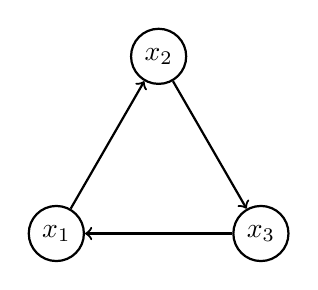
\begin{tikzpicture}[
			node distance=2cm,
			vertice/.style={circle, draw, thick, minimum size=7mm, inner sep=0pt}
			]
			\node[vertice] (x2) at (90:1.5cm) {$x_2$};
			\node[vertice] (x1) at (210:1.5cm) {$x_1$};
			\node[vertice] (x3) at (330:1.5cm) {$x_3$};
			
			\draw[->, thick] (x1) -- (x2);
			\draw[->, thick] (x2) -- (x3);
			\draw[->, thick] (x3) -- (x1);
		\end{tikzpicture}
	\end{center}
	
	\begin{proposizione}{Inesistenza dell'ordine topologico}{}
		Se il \textbf{grafo orientato} $G$ definito dai processi \textbf{contiene un ciclo diretto}, allora \textbf{non esiste} alcun ordine topologico.
	\end{proposizione}
	
	\begin{dimostrazione}{}{}
		Procediamo per assurdo. Assumiamo che esista un ciclo diretto formato dalla sequenza di vertici $(v_1, \dots, v_k)$ e che, contemporaneamente, esista un ordine topologico valido per il grafo.
		
		Se $v_i$ precede $v_{i+1}$ lungo il ciclo, allora per soddisfare la condizione di chiusura del ciclo deve esistere un arco che dal termine della sequenza ritorna all'inizio. Tuttavia, la presenza dell'arco $(v_i, v_{i+1})$ rende impossibile preservare l'ordinamento topologico lineare, poiché per definizione tutti gli archi orientati devono puntare coerentemente nella medesima direzione della sequenza (da destra verso sinistra nella notazione stabilita). Di conseguenza, almeno un arco lungo il ciclo violerà necessariamente la relazione d'ordine.
	\end{dimostrazione}
	
	\begin{proposizione}{Proprietà dei cicli nei grafi diretti}{}
		Se $\nexists$ un ciclo in un grafo diretto $\implies \exists$ un ordine topologico.
	\end{proposizione}
	
	\begin{proposizione}{Esistenza di vertici senza archi uscenti}{}
		Se $G$ è un grafo diretto senza cicli $\implies \exists$ un vertice $v$ senza archi uscenti.
	\end{proposizione}
	
	\begin{proposizione}{Presenza di cicli nei grafi diretti}{}
		Per ogni vertice $v$, se $\exists$ almeno un arco uscente da $v \implies G$ contiene un ciclo.
	\end{proposizione}
	
	\begin{definizione}{DAG (Directed Acyclic Graph)}{}
		Per notazione, indichiamo con \textbf{DAG} (\textit{Directed Acyclic Graph}) un grafo diretto privo di cicli.
	\end{definizione}
	
	\subsection{Ricerca di un ordine topologico}
	Vogliamo definire un algoritmo per trovare un \textbf{ordine topologico} in un grafo orientato aciclico (DAG).
	
	\begin{osservazione}{Proprietà fondamentale}{}
		Per la proposizione precedente, sappiamo che se in un grafo orientato esiste un ordine topologico, allora esiste \textbf{almeno un nodo senza archi uscenti} (ovvero un nodo pozzo).
	\end{osservazione}
	
	Da questa osservazione nasce l'idea per un primo algoritmo. L'idea di base consiste nell'eseguire iterativamente le seguenti operazioni:
	\begin{enumerate}
		\item Scorriamo tutti i vertici del grafo e individuiamo un vertice privo di archi uscenti.
		
		\item Lo rimuoviamo dal grafo.
		
		\item Ripetiamo il procedimento finché non sono stati rimossi tutti i vertici.
	\end{enumerate}
	
	Formalizziamo questo approccio tramite il seguente pseudo-codice:
	
	\begin{lstlisting}[style=stile-listings, caption={Algoritmo ingenuo per l'ordine topologico}]
		Ord(G: grafo diretto aciclico):
			L = []
			while len(G) != 0:
				v = trova_nodo_senza_archi_uscenti(G)
				L.append(v)
				cancella_nodo_e_archi(G, v)
			return L
	\end{lstlisting}
	
	\begin{algoritmo}{Ordine topologico (inefficiente)}{}
		Analizziamo nel dettaglio le singole istruzioni dell'algoritmo e i relativi costi computazionali:
		\begin{itemize}
			\item \textbf{Inizializzazione e ciclo principale}: Il ciclo \texttt{while} viene eseguito $\Theta(n)$ volte, poiché a ogni iterazione viene rimosso esattamente un nodo dal grafo.
			
			\item \textbf{Ricerca del nodo senza figli}: Per individuare un vertice senza archi uscenti (ovvero un nodo la cui lista di adiacenza sia vuota), dobbiamo scorrere i nodi del grafo, con un costo di $O(n)$.
			
			\item \textbf{Cancellazione del nodo}: La rimozione del nodo $v$ dal grafo e la successiva eliminazione di tutte le sue occorrenze nelle liste di adiacenza degli altri nodi richiede di scandire l'intera struttura dati, con un costo pari a $O(n + m)$.
		\end{itemize}
		
		Il costo totale dell'algoritmo risulta quindi essere:
		\[
		\Theta(n) \cdot O(n + m) = O(n(n + m))
		\]
	\end{algoritmo}
	
	\begin{osservazione}{Presenza di più nodi pozzo}{}
		Anche se nel grafo dovessero essere presenti più nodi contemporaneamente privi di archi uscenti, l'algoritmo funziona correttamente. Esso restituirà comunque un ordine topologico valido (ricordando che per uno stesso DAG possono esistere più ordini topologici distinti).
	\end{osservazione}
	
	Come si nota dall'analisi della complessità, si tratta di un metodo \textbf{molto costoso} dal punto di vista computazionale, oltre al fatto che modifica in modo distruttivo la struttura del grafo originale.
	
	\begin{esercizio}{Trovare un ciclo in un grafo diretto}{}
		Dato un grafo diretto G, trovare un ciclo al suo interno.
	\end{esercizio}
	
	\begin{lstlisting}[style=stile-listings, language=Python, caption={Algoritmo per la ricerca di un ciclo diretto}]
		def trovaCicloDiretto(G):
			L = []  # Per memorizzare i nodi del ciclo
			x = vertice qualsiasi
			L.append(x)
			
			vis = [0] * n
			vis[x] = 1  # Segniamo il nodo come visitato
			
			current = x
			next = x.neighbr[0]
			
			# Iteriamo finche non troviamo un nodo gia visitato
			while vis[next] == 0:
				vis[next] = 1
				L.append(next)
				
				current = next
				next = current.neighbr[0]  # (1)
				
			while L[0] != next:
				L.remove()
			
			return L
	\end{lstlisting}
	
	\begin{algoritmo}{Ricerca di un ciclo diretto}{}	
		\begin{enumerate}
			\item \textbf{Inizializzazione}: Viene creata una lista $L$ per memorizzare il percorso e un vettore di tracciamento \texttt{vis} di dimensione $n$ inizializzato a $0$. Si seleziona un vertice di partenza arbitrario $x$, lo si inserisce in $L$ e si imposta \texttt{vis[x] = 1}.
			\item \textbf{Esplorazione}: Si imposta \texttt{current = x} e come vertice successivo \texttt{next} il primo adiacente uscente (\texttt{x.neighbr[0]}).
			\item \textbf{Ricerca del ciclo}: Finché il nodo \texttt{next} non è stato visitato (\texttt{vis[next] == 0}):
			\begin{itemize}
				\item Si marca \texttt{next} come visitato (\texttt{vis[next] = 1}).
				\item Si aggiunge \texttt{next} alla lista $L$.
				\item Si avanza ponendo \texttt{current = next} e selezionando il nuovo vicino uscente \texttt{next = current.neighbr[0]} (istruzione \textbf{(1)}).
			\end{itemize}
			\item \textbf{Estrazione della sequenza del ciclo}: Quando il ciclo \texttt{while} termina, significa che \texttt{next} è un nodo già visitato (è stato ri-incontrato). Il secondo ciclo \texttt{while} rimuove gli elementi in testa a $L$ finché l'elemento di testa non coincide con \texttt{next}, lasciando in $L$ solo ed esclusivamente i nodi che compongono il ciclo diretto trovato.
		\end{enumerate}
		
		L'unica sostanziale differenza rispetto al caso non orientato è un'accortezza: nell'istruzione \textbf{(1)} possiamo permetterci di assegnare come prossimo nodo sempre il primo dei vicini (\texttt{current.neighbr[0]}). Infatti, essendo il grafo \textbf{diretto}, anche la presenza di un eventuale doppio arco orientato tra due soli nodi costituisce a tutti gli effetti un ciclo valido.
	\end{algoritmo}
	
	\begin{esercizio}{Problema dell'antenato comune più vicino}{}
		Dato $P$ il vettore dei padri di un albero e dati due vertici $x$ ed $y$, l'obiettivo è trovare l'antenato comune più vicino (noto anche come Lowest Common Ancestor o LCA) tra $x$ e $y$.
	\end{esercizio}
	
	Presentiamo una soluzione basata sull'utilizzo di liste puntate per risalire la gerarchia dei padri fino alla radice.
	
	\begin{lstlisting}[style=stile-listings]
		def sol1(P, x, y):
			L1, L2 liste puntate
			Do:
				L1.push(x)
				x = P[x]
			while x != P[x]
			
			Do:
				L2.push(y)
				y = P[y]
			while y != P[y]
			
			Current = L1[0]
			while L1[1] == L2[1]:
				Current = L1[1]
				L1.remove()
				L2.remove()
			
			return Current
	\end{lstlisting}
	
	\begin{osservazione}{}{}
		Essendo \texttt{L1} ed \texttt{L2} liste puntate, gli elementi vengono aggiunti in testa durante la risalita verso la radice. Di conseguenza, alla fine dell'inserimento, il primo elemento della lista corrisponde proprio alla radice dell'albero, mentre gli ultimi elementi rappresentano i nodi di partenza $x$ ed $y$.
	\end{osservazione}
	
	Tornando agli ordini topologici...
	In precedenza era stata presentata una versione inefficiente con complessità temporale pari a $O(n(n+m))$. È possibile progettare una versione decisamente più efficiente sfruttando una visita in profondità (\textbf{DFS}). 
	
	Prima di definire formalmente l'algoritmo, introduciamo alcune nozioni teoriche fondamentali relative alla gestione del tempo durante la visita.
	
	\begin{definizione}{Tempi di scoperta e fine visita in DFS}{}
		Dato un grafo $G$ e una visita DFS su di esso, introduciamo un \textbf{contatore globale che viene incrementato ad ogni nuovo nodo visitato}. Ad ogni nodo $v$ viene associata una coppia di valori temporali:
		\begin{itemize}
			\item \textbf{Tempo di scoperta} $t(v)$: indica il valore del contatore nel momento in cui il nodo $v$ viene inserito nello stack della DFS. Sostanzialmente, rappresenta l'istante in cui il vertice viene visitato per la prima volta.
			\item \textbf{Tempo di fine visita} $T(v)$: indica il valore del contatore nel momento in cui il nodo $v$ viene rimosso dallo stack della DFS. Sostanzialmente, indica quanti nodi sono stati esplorati complessivamente prima di eliminare $v$ dallo stack (ovvero quando l'esplorazione di $v$ e di tutti i suoi discendenti è terminata).
		\end{itemize}
	\end{definizione}
	
	\begin{center}
		\begin{tikzpicture}[
			scale=1.2,
			nodo/.style={circle, draw=black, thick, minimum size=6mm, inner sep=0pt, font=\bfseries},
			arco/.style={->, >=stealth, thick},
			intervallo/.style={text=DarkGoldenrod3, font=\small\bfseries}
			]
			% Definizione dei vertici
			\node[nodo] (1) at (0, 1.5) {1};
			\node[nodo] (4) at (2, 3) {4};
			\node[nodo] (3) at (5, 3) {3};
			\node[nodo] (2) at (3.5, 1.5) {2};
			\node[nodo] (5) at (5, -0.5) {5};
			
			% Intervalli associati ai nodi
			\node[intervallo, below left=2pt and 0pt of 1] {$[1, 5]$};
			\node[intervallo, above left=2pt and 0pt of 4] {$[2, 3]$};
			\node[intervallo, above right=2pt and 0pt of 3] {$[3, 3]$};
			\node[intervallo, right=1.2cm of 2] (lbl2) {$[4, 5]$};
			\draw[->, DarkGoldenrod3, thick] (lbl2) -- (2);
			\node[intervallo, right=4pt of 5] (lbl5) {$[5, 5]$};
			
			% Nota per il nodo 5
			\node[DarkOrchid3, font=\footnotesize, align=left, above right=0.3cm and 0.5cm of 5] (nota5) {perché non ha archi\\uscenti su nodi ``nuovi''};
			\draw[->, DarkOrchid3, thick] (nota5) to[out=190, in=120] (lbl5);
			
			% Archi orientati
			\draw[arco] (1) -- (4);
			\draw[arco] (1) -- (2);
			\draw[arco] (1) -- (5);
			\draw[arco] (4) -- (3);
			\draw[arco] (2) -- (4);
			\draw[arco] (2) -- (3);
			\draw[arco] (2) -- (5);
			\draw[arco] (5) -- (3);
		\end{tikzpicture}
	\end{center}
	
	Consideriamo il grafo sopra rappresentato ed analizziamo l'evoluzione della visita in profondità (DFS):
	\begin{enumerate}
		\item \textbf{Partenza dal nodo radice}: supponiamo di partire dal nodo $1$. Poniamo $t(1) = 1$, in quanto è il primo vertice visitato.
		\item \textbf{Attraversamento di un arco uscente}: scegliamo un arco uscente arbitrario, ad esempio verso il nodo $4$. Poniamo $t(4) = 2$, essendo il secondo vertice visitato.
		\item \textbf{Avanzamento}: ci muoviamo verso l'unico nodo adiacente disponibile, il nodo $3$, e poniamo $t(3) = 3$.
		\item \textbf{Backtracking da nodo senza uscite non visitate}: poiché il nodo $3$ non possiede archi uscenti verso nodi ancora da scoprire, lo rimuoviamo dallo stack per effettuare il backtracking. Poniamo quindi $T(3) = 3$. Si noti che si tratta dello stesso contatore, ma in questo passaggio non viene incrementato.
		\item \textbf{Ritorno al predecessore}: torniamo al nodo $4$; dato che non ha altri archi uscenti verso nodi non ancora visitati, lo eliminiamo dallo stack e assegniamo $T(4) = 3$.
		\item \textbf{Prosecuzione}: si procede in modo analogo per i restanti vertici del grafo.
	\end{enumerate}
	
	Da questo meccanismo possiamo ricavare due proprietà fondamentali sui tempi di scoperta e di fine visita:
	
	\begin{osservazione}{Tempi della radice}{}
		Se il grafo è connesso e $v$ è la radice dell'albero di visita, si ha necessariamente:
		\[
		t(v) = 1, \qquad T(v) = n
		\]
		Ciò è dovuto al fatto che la radice è il primo nodo ad essere scoperto ed è l'ultimo ad essere rimosso dallo stack.
	\end{osservazione}
	
	\begin{osservazione}{Relazione tra tempo di inizio e fine visita}{}
		Per ogni vertice $v \in V$ vale la disuguaglianza:
		\[
		t(v) \le T(v)
		\]
		in quanto un nodo deve essere necessariamente scoperto prima di poter terminare la sua elaborazione ed essere rimosso.
	\end{osservazione}
	
	Dunque, ad ogni vertice $v$ risulta associato un intervallo temporale ben definito:
	\[
		[t(v), T(v)]
	\]
	
	\begin{proposizione}{Classificazione degli archi in una DFS}{classificazione_archi}
		Per ogni coppia di vertici $u, v$, con $u$ la coda dell'arco e $v$ la testa, vale solo una di queste relazioni:
		\begin{itemize}
			\item[\textbf{i)}] $[t(u), T(u)] \subseteq [t(v), T(v)]$ : \textbf{ARCO ALL'INDIETRO}
			\item[\textbf{ii)}] $[t(v), T(v)] \subseteq [t(u), T(u)]$ : \textbf{ARCO IN AVANTI}
			\item[\textbf{iii)}] $[t(u), T(u)] \cap [t(v), T(v)] = \emptyset$ : \textbf{ARCO DI ATTRAVERSAMENTO}
		\end{itemize}
	\end{proposizione}
	
	\begin{minipage}[c]{0.55\textwidth}
		\centering
		\begin{tikzpicture}[
			scale=1.3,
			vertex/.style={circle, draw, minimum size=18pt, thick, fill=white},
			edge/.style={->, >=stealth, thick}
			]
			% Nodi
			\node[vertex] (v1) at (0,1) {1};
			\node[vertex] (v4) at (1.5,2.2) {4};
			\node[vertex] (v3) at (3.5,2.2) {3};
			\node[vertex] (v2) at (2,0.8) {2};
			\node[vertex] (v5) at (3.5,-1) {5};
			
			% Etichette intervalli (arancione)
			\node[orange, left=0.15cm of v1] {\textbf{[1, 5]}};
			\node[orange, above left=0.05cm of v4] {\textbf{[2, 3]}};
			\node[orange, above right=0.05cm of v3] {\textbf{[3, 3]}};
			\node[orange, right=0.8cm of v2] (lbl2) {\textbf{[4, 5]}};
			\draw[orange, ->, thick] (lbl2) -- (v2);
			\node[orange, right=0.15cm of v5] {\textbf{[5, 5]}};
			
			% Archi
			\draw[edge] (v1) -- (v4);
			\draw[edge] (v4) -- (v3);
			\draw[edge] (v1) -- (v2);
			\draw[edge] (v2) -- (v3);
			\draw[edge] (v2) -- (v5);
			\draw[edge] (v5) -- (v3);
			\draw[edge] (v5) -- (v1);
			\draw[edge] (v2) -- (v4);
		\end{tikzpicture}
	\end{minipage}
	\begin{minipage}[c]{0.4\textwidth}
		\textbf{In questo esempio abbiamo:}
		\begin{itemize}
			\item $(1, 4) = $ \textbf{\color{MediumOrchid3}AVANTI}
			\item $(4, 3) = $ \textbf{\color{MediumOrchid3}AVANTI}
			\item $(1, 2) = $ \textbf{\color{MediumOrchid3}AVANTI}
			\item $(2, 3) = $ \textbf{\color{Coral3}ATTRAVERSAMENTO}
			\item $(2, 5) = $ \textbf{\color{MediumOrchid3}AVANTI}
			\item $(5, 3) = $ \textbf{\color{Coral3}ATTRAVERSAMENTO}
			\item $(5, 1) = $ \textbf{\color{DarkGoldenrod2}INDIETRO}
			\item $(2, 4) = $ \textbf{\color{Coral3}ATTRAVERSAMENTO}
		\end{itemize}
	\end{minipage}
	
	\vspace{2em}
	
	Ragionando tenendo conto dell'arborescenza, cioè dell'albero delle visite che si crea dalla successione dei nodi che appaiono in una DFS su un grafo diretto, vediamo come:
	
	\begin{itemize}
		\item \textbf{ARCHI IN AVANTI:} archi che vanno da un nodo ad un suo \textbf{discendente}.
		\item \textbf{ARCHI ALL'INDIETRO:} archi che vanno da un nodo ad un suo \textbf{antenato}.
		\item \textbf{ARCHI DI ATTRAVERSAMENTO:} archi che vanno da un nodo ad un suo \textbf{"cugino"}.
	\end{itemize}
	
	\begin{dimostrazione}{}{}
		Per dimostrare che vale almeno una di queste proprietà, è necessario dimostrare che \textbf{non esiste} alcun caso in cui i due intervalli si sovrappongono parzialmente.
		
		\begin{center}
			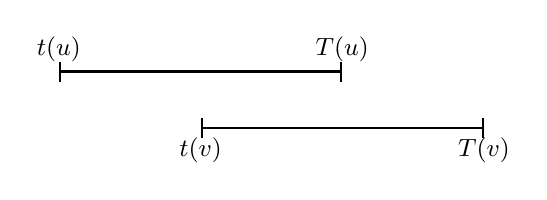
\begin{tikzpicture}[scale=1.2, every node/.style={font=\small}]
				% Primo intervallo (u)
				\draw[thick, |-|] (0, 0.6) -- (3, 0.6);
				\node[above] at (0, 0.6) {$t(u)$};
				\node[above] at (3, 0.6) {$T(u)$};
				
				% Secondo intervallo (v)
				\draw[thick, |-|] (1.5, 0) -- (4.5, 0);
				\node[below] at (1.5, 0) {$t(v)$};
				\node[below] at (4.5, 0) {$T(v)$};
			\end{tikzpicture}
		\end{center}
		
		Cioè, una situazione in cui $t(u) < t(v) \le T(u) < T(v)$ è \textbf{impossibile}.
		
		Supponiamo che $u$ sia il nodo inserito per primo nello stack. Di conseguenza, deve valere necessariamente $t(u) < t(v)$, dato che $v$ viene visitato successivamente.
		
		Per la natura LIFO (Last In, First Out) dello stack, il nodo $v$ deve essere rimosso prima di $u$, poiché l'ultimo elemento a essere visitato deve essere anche il primo a essere rimosso. Siccome $v$ viene sicuramente rimosso prima di $u$, è \textbf{impossibile} che si verifichi $T(v) > T(u)$.
	\end{dimostrazione}
	
	\section{Comportamento nei grafi non diretti}
	
	Come si comporta questa implementazione nei \textbf{grafi non diretti}?
	
	Siccome il grafo non è orientato, si possono verificare solo due possibili casi per gli intervalli di visita di qualsiasi coppia di nodi $u, v$:
	\begin{itemize}
		\item[\textbf{i/ii)}] $I_u \subseteq I_v$ oppure $I_v \subseteq I_u$
		\item[\textbf{iii)}] $I_u \cap I_v = \emptyset$
	\end{itemize}
	
	\begin{center}
		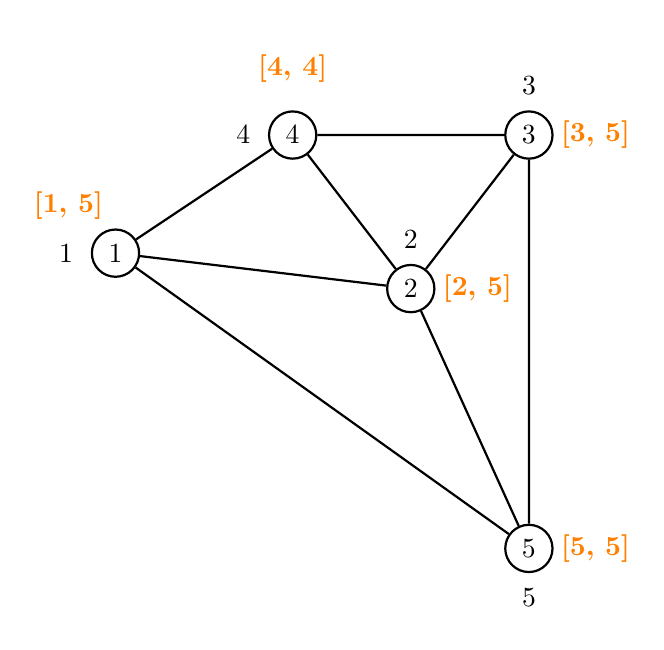
\begin{tikzpicture}[scale=1.5, every node/.style={circle, draw, minimum size=6mm, inner sep=1pt, thick}]
			% Nodi con etichette nere e intervalli arancioni
			\node (n1) at (0, 1.5) [label=above left:{\color{orange}\textbf{[1, 5]}}, label=left:1] {1};
			\node (n4) at (1.5, 2.5) [label=above:{\color{orange}\textbf{[4, 4]}}, label=left:4] {4};
			\node (n3) at (3.5, 2.5) [label=right:{\color{orange}\textbf{[3, 5]}}, label=above:3] {3};
			\node (n2) at (2.5, 1.2) [label=right:{\color{orange}\textbf{[2, 5]}}, label=above:2] {2};
			\node (n5) at (3.5, -1) [label=right:{\color{orange}\textbf{[5, 5]}}, label=below:5] {5};
			
			% Archi
			\draw[thick] (n1) -- (n4);
			\draw[thick] (n1) -- (n2);
			\draw[thick] (n1) -- (n5);
			\draw[thick] (n4) -- (n3);
			\draw[thick] (n4) -- (n2);
			\draw[thick] (n3) -- (n2);
			\draw[thick] (n3) -- (n5);
			\draw[thick] (n2) -- (n5);
		\end{tikzpicture}
		\par\vspace{0.5em}
		\textit{\color{purple}Nota: possiamo scegliere noi un ordine di visita dei nodi, di conseguenza l'intervallo segnato nel grafo è riportato solo a scopo esemplificativo.}
	\end{center}
	
	\begin{proposizione}{}{}
		Dato un DFS su un grafo \textbf{non diretto}, se un arco $(u, v)$ non fa parte dell'\textbf{albero di visita} (ovvero è un arco all'indietro/back edge), allora è impossibile che si verifichi il caso \textbf{iii)} degli intervalli disgiunti.
	\end{proposizione}
	
	\begin{dimostrazione}{}{}
		Supponiamo per assurdo che gli intervalli siano disgiunti, ovvero che esista un arco $(u, v)$ tale che:
		\[
		I_u \cap I_v = \emptyset
		\]
		Sicuramente uno dei due nodi verrà visitato prima dell'altro; senza perdita di generalità, assumiamo che questo sia $u$, ovvero che $t(u) < t(v)$.
		
		Data questa assunzione e data la natura LIFO dello stack, è impossibile che $u$ venga rimosso dallo stack prima che inizi la visita di $v$, poiché l'esistenza dell'arco $(u, v)$ impone che $v$ venga scoperto prima della chiusura di $u$. Di conseguenza, deve valere:
		\[
		t(v) \le T(u)
		\]
		Il che dimostra che gli intervalli non sono disgiunti, giungendo a una contraddizione.
	\end{dimostrazione}
	
	\begin{osservazione}{Archi fuori dall'albero in grafi non orientati}{}
		Tutti gli archi $(u, v)$ che non fanno parte dell'albero di visita di una DFS su un grafo non orientato sono necessariamente \textbf{archi all'indietro} (o in avanti; non essendoci un orientamento nel grafo, la distinzione non è rilevante).
	\end{osservazione}
	
	\begin{proposizione}{Caratterizzazione dei cicli in grafi non orientati}{}
		Sia $G$ un grafo non orientato connesso.
		\[
		G \text{ ha un ciclo} \iff \text{ogni DFS ha almeno un arco all'indietro}
		\]
	\end{proposizione}
	
	\begin{dimostrazione}{}{}
		Analizziamo le due direzioni della doppia implicazione:
		\begin{itemize}
			\item \textbf{Direzione} ``$\implies$'':\\
			Abbiamo osservato in precedenza che tutti gli archi che non appartengono all'albero di visita DFS sono archi all'indietro. Dato un ciclo $C$ nel grafo, ed essendo l'albero di visita un grafo aciclico connesso per definizione, deve necessariamente esistere almeno un arco di $C$ che non appartiene all'albero. Tale arco sarà quindi un arco all'indietro.
			
			\item \textbf{Direzione} ``$\impliedby$'':\\
			Sia $(u, v)$ un arco all'indietro, con $u$ discendente di $v$ nell'albero DFS. Per definizione di discendenza, nell'albero di visita esiste un cammino $P$ da $v$ a $u$. Di conseguenza, l'unione del cammino $P$ con l'arco all'indietro $(u, v)$ forma un ciclo nel grafo.
		\end{itemize}
	\end{dimostrazione}
	
	\begin{proposizione}{Caratterizzazione dei cicli in grafi orientati}{}
		Dato un grafo orientato $G$:
		\[
		\exists \text{ un ciclo in } G \iff \exists \text{ un arco all'indietro per qualsiasi DFS nel grafo}
		\]
	\end{proposizione}
	
	\begin{dimostrazione}{}{}
		Analizziamo le due direzioni della doppia implicazione:
		\begin{itemize}
			\item \textbf{Direzione} ``$\impliedby$'':\\
			Supponiamo che esista un arco all'indietro $(u, v)$, il che implica che $u$ è un discendente di $v$ nell'albero DFS. Nell'albero delle visite esiste quindi un cammino diretto $v \to u$. L'unione di tale cammino con l'arco diretto $(u, v)$ costituisce un ciclo diretto nel grafo.
			
			\item \textbf{Direzione} ``$\implies$'':\\
			Sia $C$ un ciclo nel grafo $G$ e sia $v$ il primo vertice di $C$ ad essere visitato dalla DFS. Di conseguenza, tutti gli altri vertici del ciclo $C$ verranno scoperti mentre $v$ è ancora attivo, diventando quindi discendenti di $v$ nell'albero DFS.
			
			Il vertice $v_k$ che completa il ciclo e si ricongiunge con $v$ darà origine a un arco $(v_k, v)$ che si configura come un arco all'indietro.
			
			Questo comportamento è garantito per tutti i nodi $u$ del ciclo visitati dopo $v$, in quanto, trovandosi all'interno del ciclo ed essendo stati scoperti dopo $v$, verranno terminati (e quindi rimossi dallo stack di ricorsione) prima di $v$. In termini di tempi di scoperta $t$ e fine visita $T$:
			\[
			t(v) < t(u) \land T(v) > T(u) \quad \forall u \in C \setminus \{v\}
			\]
		\end{itemize}
	\end{dimostrazione}
	
	Torniamo molto a monte: vogliamo usare tutte queste supposizioni per dare un codice per trovare l'ordine topologico in un tempo $O(n+m)$ usando la DFS.
	
	Programmiamo ora una DFS ricorsiva che ci permette di ottenere $t[x]$ e $T[x]$ per ogni vertice.
	
	\begin{lstlisting}[style=stile-listings, language=Python]
		def DFS_ric(G, x, t, T, c):
			for y in x.neighbor:
				if t[y] == -1:
					c += 1
					t[y] = c
					DFS_ric(G, y, t, T, c)
			T[x] = c
		
		def DFS(G, x):
			t = [-1] * n
			T = [-1] * n
			c = 1
			t[x] = c
			DFS_ric(G, x, t, T, c)
	\end{lstlisting}
	
	\begin{algoritmo}{Ricerca in profondità (DFS) con tempi di visita}{}
		La seguente procedura implementa la visita DFS tenendo traccia dei tempi di scoperta $t[x]$ e di fine visita $T[x]$ per ciascun vertice $x$.
		
		\paragraph{Spiegazione dettagliata delle istruzioni:}
		\begin{itemize}
			\item \textbf{Controllo della visita (\texttt{t[y] == -1}):} Usiamo l'array $t$ per controllare se abbiamo già visitato il vertice $y$. Poiché $t[y]$ indica il tempo in cui abbiamo scoperto $y$, un valore pari a $-1$ indica che il nodo non è ancora stato visitato.
			
			\item \textbf{Fine visita del sottoalbero (\texttt{T[x] = c}):} Una volta che abbiamo visitato tutto il sottoalbero di $x$, dobbiamo rimuoverlo dallo stack e andare avanti, dunque valorizziamo il tempo di fine visita $T[x]$ con il valore corrente del contatore $c$ (questo avviene in quanto non stiamo usando uno stack esplicito, bensì lo stack della ricorsione delle chiamate di funzione: la risalita dello stack della ricorsione corrisponde alla rimozione graduale dei nodi dallo stack).
			
			\item \textbf{Inizializzazione:} Nella funzione principale \texttt{DFS(G, x)} inizializziamo i due array $t$ e $T$ di dimensione $n$ con il valore $-1$, impostiamo il contatore iniziale $c = 1$, marchiamo il nodo di partenza $x$ e infine avviamo la procedura ricorsiva.
		\end{itemize}
	\end{algoritmo}
	
	Per l'ordine topologico sappiamo che non ci sono archi all'indietro, essendo il grafo aciclico (DAG).
	
	Di conseguenza, per qualsiasi arco $(u, v)$, vale esclusivamente una delle seguenti relazioni tra gli intervalli temporali di visita:
	\begin{itemize}
		\item \textbf{Disgiunzione:}
		\[
		[t[v], T[v]] \cap [t[u], T[u]] = \emptyset
		\]
		\item \textbf{Inclusione:}
		\[
		[t[v], T[v]] \subseteq [t[u], T[u]]
		\]
		In questo caso, l'arco $(u, v)$ rappresenta un arco in avanti oppure un arco di \textbf{arborescenza}.
	\end{itemize}
	
	Dunque, per ogni arco $(u, v)$ del grafo, vale sempre la relazione:
	\[
	T[v] \le T[u]
	\]
	% --- NEW PAGE (26) ---
	
	Per ricostruire un ordinamento topologico, dobbiamo considerare l'array dei tempi di fine visita $T$ in ordine decrescente: infatti, l'ultimo vertice ad essere completato nella visita è il primo nell'ordine topologico.
	
	\begin{center}
		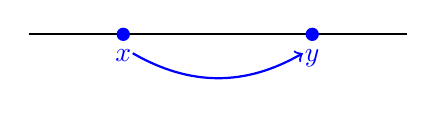
\begin{tikzpicture}[scale=1.2]
			\draw[thick] (0, 0) -- (4, 0);
			\fill[blue] (1, 0) circle (2pt) node[below=2pt] {$x$};
			\fill[blue] (3, 0) circle (2pt) node[below=2pt] {$y$};
			\draw[->, thick, blue] (1.1, -0.2) to[out=-30, in=-150] (2.9, -0.2);
		\end{tikzpicture}
		\par\vspace{0.3em}
		{\small Con un arco che collega $x$ e $y$, si ha $T[y] \le T[x]$ e quindi l'arco è orientato come $x \to y$.}
	\end{center}
	
	Se invece consideriamo i tempi di fine visita $T$ in ordine crescente, il primo vertice ad essere rimosso risulterà essere l'ultimo nell'ordinamento topologico.
	
	\begin{center}
		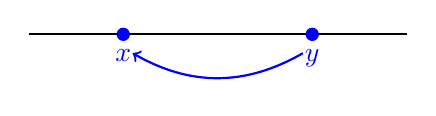
\begin{tikzpicture}[scale=1.2]
			\draw[thick] (0, 0) -- (4, 0);
			\fill[blue] (1, 0) circle (2pt) node[below=2pt] {$x$};
			\fill[blue] (3, 0) circle (2pt) node[below=2pt] {$y$};
			\draw[->, thick, blue] (2.9, -0.2) to[out=-150, in=-30] (1.1, -0.2);
		\end{tikzpicture}
		\par\vspace{0.3em}
		{\small Con un arco che collega $x$ e $y$, si ha $T[y] \ge T[x]$ e quindi l'arco è orientato come $y \to x$.}
	\end{center}
	
	Abbiamo dunque tutti gli elementi teorici necessari per definire l'algoritmo di ordinamento topologico basato su DFS.
	
	\begin{lstlisting}[style=stile-listings, language=Python]
		def OrdTop(G):
			L = []
			vis = [0] * n
			for v in G:
				if vis[v] == 0:
					OrdTopRic(G, v, vis, L)
			return L
		
		def OrdTopRic(G, v, vis, L):
			vis[v] = 1
			for u in v.neighbors:
				if vis[u] == 0:
					OrdTopRic(G, u, vis, L)
			L.append(v)
	\end{lstlisting}
	
	\begin{algoritmo}{Ordinamento Topologico}{ord_top}
		\begin{itemize}
			\item \textbf{Inizializzazione (\texttt{OrdTop}):} viene predisposta una lista $L$ inizialmente vuota per raccogliere i nodi ordinati e un vettore booleano \texttt{vis} di dimensione $n$ inizializzato a $0$, impiegato per tracciare lo stato di visita di ciascun vertice.
			
			\item \textbf{Ciclo principale:} per ogni vertice $v \in G$, se $v$ non è ancora stato visitato (\texttt{vis[v] == 0}), si avvia la procedura ricorsiva \texttt{OrdTopRic(G, v, vis, L)}. Al termine delle chiamate per tutte le componenti connesse, viene restituita la lista $L$.
			
			\item \textbf{Procedura ricorsiva (\texttt{OrdTopRic}):}
			\begin{enumerate}
				\item Il vertice corrente $v$ viene marcato come visitato impostando \texttt{vis[v] = 1}.
				
				\item Si esaminano tutti i vertici $u$ uscenti da $v$ (\texttt{v.neighbors}): se un vicino $u$ non è ancora stato visitato (\texttt{vis[u] == 0}), la funzione richiama ricorsivamente se stessa su $u$.
				
				\item Non appena tutti i discendenti di $v$ sono stati esplorati (visita in post-ordine), il nodo $v$ viene inserito in $L$ tramite l'operazione \texttt{L.append(v)}. L'inserimento del vertice $v$ come ultimo elemento della lista è un modo molto furbo di utilizzare la risalita dello stack della ricorsione per inserire per ultimo letteralmente \textit{l'ultimo vertice a cui siamo arrivati}, ovvero quello con la priorità minore (l'ultimo dell'ordine topologico).
			\end{enumerate}
		\end{itemize}
	\end{algoritmo}
	
	La procedura richiama perfettamente una classica operazione di DFS, dunque il costo computazionale sarà $\mathbf{O(n + m)}$.
	
	\begin{definizione}{Pozzo universale}{}
		In un grafo diretto $G$, un \textbf{pozzo universale} è un vertice $x \in V(G)$ tale che:
		\[
		\forall y \in V(G) \setminus \{x\}, \quad (y, x) \in E(G) \land (x, y) \notin E(G)
		\]
		In termini intuitivi, si tratta di un nodo a cui arrivano archi da tutti gli altri vertici del grafo, ma dal quale non parte alcun arco verso l'esterno.
	\end{definizione}
	
	\begin{esercizio}{Ricerca del pozzo universale in tempo}{}
		Dato un grafo $G$ con $n$ vertici memorizzato tramite una matrice di adiacenza, l'obiettivo è stabilire se esiste un pozzo universale in tempo lineare $O(n)$.
		
		\paragraph{Idea intuitiva}
		La matrice di adiacenza ci permette di verificare la presenza di un arco tra due nodi $i$ e $j$ in tempo costante $O(1)$. Da un singolo controllo sulla cella $G[i][j]$ possiamo ricavare due informazioni cruciali che ci consentono di escludere uno dei due nodi come potenziale pozzo:
		\begin{itemize}
			\item \textbf{Se $G[i][j] == 0$}: significa che non esiste un arco orientato da $i$ a $j$. Di conseguenza, $j$ \textbf{non può} essere un pozzo universale, poiché un pozzo universale deve essere raggiunto da tutti gli altri nodi del grafo (incluso $i$).
			
			\item \textbf{Se $G[i][j] == 1$}: significa che esiste un arco orientato da $i$ a $j$. Di conseguenza, $i$ \textbf{non può} essere un pozzo universale, poiché da un pozzo universale non deve partire alcun arco verso l'esterno.
		\end{itemize}
		Grazie a questa proprietà, con un singolo confronto siamo in grado di scartare un candidato, riducendo progressivamente lo spazio di ricerca.\\
		Inoltre, per la definizione di pozzo universale, possiamo ricavare un'altra informazione dalla matrice di adiacenza.
		\begin{itemize}
			\item La riga di indice \texttt{candidato\_pozzo} deve essere interamente composta da 0, in quanto dal pozzo non devono partire archi.
			
			\item La colonna di indice \texttt{candidato\_pozzo} deve essere interamente composta da 1 (fatta eccezione per l'elemento \texttt{G[candidato][candidato]}, in quanto elemento della diagonale e dato che non stiamo ammettendo archi riflessivi).
		\end{itemize}
	\end{esercizio}
	
	\begin{lstlisting}[style=stile-listings, language=Python]
		def trovaPozzo(G):
			i, j = 1, 2
			candidato = 1
			n = len(G)
			
			while i <= n and j <= n:
				if G[i][j] == 0:
					j += 1
					candidato = i
				else:
					i += 1
					candidato = j
			
			for k in range(1, n + 1):
				if candidato == k:
					continue
				if G[k][candidato] != 1:
					return null
				if G[candidato][k] != 0:
					return null
			
			return candidato
	\end{lstlisting}
	
	\begin{algoritmo}{Ricerca di un pozzo in tempo $O(n)$}{}
		\begin{enumerate}
			\item \textbf{Fase di eliminazione (righe 2-13)}:
			\begin{itemize}
				\item Vengono inizializzati due indici $i = 1$ e $j = 2$ per scorrere la matrice di adiacenza, e una variabile \texttt{candidato = 1} per memorizzare il nodo che attualmente potrebbe essere il pozzo.
				\item Nel ciclo \texttt{while}, finché entrambi gli indici sono entro i limiti della matrice ($i \le n$ e $j \le n$), si effettua il controllo sulla cella $G[i][j]$.
				\item Se $G[i][j] == 0$, escludiamo $j$ incrementando il suo indice ($j\texttt{++}$) e impostiamo il nuovo \texttt{candidato} a $i$.
				\item Se $G[i][j] == 1$, escludiamo $i$ incrementando il suo indice ($i\texttt{++}$) e impostiamo il nuovo \texttt{candidato} a $j$.
				\item Al termine del ciclo, la variabile \texttt{candidato} conterrà l'unico nodo superstite che può effettivamente essere un pozzo universale.
			\end{itemize}
			
			\item \textbf{Fase di verifica (righe 15-21)}:
			\begin{itemize}
				\item Poiché la prima fase garantisce solo che \texttt{candidato} sia l'unico possibile pozzo (ma non che lo sia effettivamente), è necessario effettuare una verifica finale in tempo $O(n)$.
				\item Si scorre ogni nodo $k$ del grafo (escludendo il candidato stesso):
				\begin{itemize}
					\item Si controlla che esista l'arco da $k$ al candidato ($G[k][\text{\texttt{candidato}}] == 1$). Se manca anche solo un arco entrante, l'algoritmo fallisce ritornando \texttt{null}.
					\item Si controlla che non esista alcun arco dal candidato a $k$ ($G[\text{\texttt{candidato}}][k] == 0$). Se viene trovato un arco uscente, l'algoritmo fallisce ritornando \texttt{null}.
				\end{itemize}
				\item Se tutti i controlli hanno esito positivo, il \texttt{candidato} è confermato come pozzo universale e viene restituito (riga 23).
			\end{itemize}
		\end{enumerate}	
	\end{algoritmo}
	
\end{document}